\documentclass{article}

\usepackage{geometry}

\usepackage{amsmath}
\usepackage{amsfonts}
\usepackage{amssymb}
\usepackage[T1, T2A]{fontenc}
\usepackage[utf8]{inputenc}
\usepackage[english, russian]{babel}
\usepackage{graphics}
\usepackage{amsthm}
\usepackage{hyperref}
\usepackage{fancyhdr}
\usepackage{wrapfig}
\usepackage[dvips]{graphicx}
\graphicspath{{img/}}
\usepackage{float}
\usepackage{cancel}
\usepackage{fancybox}
\usepackage{caption}

\captionsetup{justification=raggedright,singlelinecheck=false}

\hypersetup{
colorlinks,
citecolor=black,
filecolor=black,
linkcolor=black,
urlcolor=black
}

\geometry{
a4paper,
total={170mm,260mm},
left=20mm,
top=20mm,
}

\newenvironment{fl*}
 {\setlength{\abovedisplayskip}{0pt}\setlength{\belowdisplayskip}{0pt}%
  \csname flalign*\endcsname}
 {\csname endflalign*\endcsname\ignorespacesafterend}

\newenvironment{fl}
 {\setlength{\abovedisplayskip}{0pt}\setlength{\belowdisplayskip}{0pt}%
  \csname flalign\endcsname}
 {\csname endflalign*\endcsname\ignorespacesafterend}

\renewcommand{\v}[1]{{\overline{#1}}}
\newcommand{\dv}[1]{\dot{\v{#1}}}
\newcommand{\norm}[1]{{\parallel #1 \parallel}}
\newcommand{\abs}[1]{{\left| #1 \right|}}
\newcommand{\R}{\mathbb{R}}
\newcommand{\pd}[2]{\frac{\partial #1}{\partial #2}}
\newcommand{\pdd}[2]{\frac{\partial}{\partial #2} \left(#1\right)}

\newcounter{lecturesCounter}
\newcommand{\lline}[1]{\subsection*{
\centering\stepcounter{lecturesCounter}\underline{Лекция \arabic{lecturesCounter} от #1}}}

\allowdisplaybreaks

\DeclareMathOperator{\grad}{grad}
\DeclareMathOperator{\rot}{rot}
\DeclareMathOperator{\rank}{rank}
\DeclareMathOperator{\diag}{diag}
\DeclareMathOperator{\re}{Re}
\DeclareMathOperator{\tr}{tr}
\DeclareMathOperator{\Div}{div}
% \DeclareMathOperator{\tg}{tg}

\newtheorem*{df}{Определение}
\newtheorem*{teo}{Теорема}
\newtheorem{lem}{Лемма}
\newtheorem{prp}{Предложение}
\newtheorem{hyp}{Предположение}
\newtheorem*{ass}{Утверждение}
\newtheorem*{cor}{Следствие}
\newtheorem*{ntc}{Замечание}
\newtheorem*{xmp}{Пример}

\renewcommand\qedsymbol{$\blacksquare$}


% \setcounter{secnumdepth}{0}
\setcounter{tocdepth}{2}

\author{Муницына Мария Александровна}
\title{Лекции по аналитической механике. Весенний семестр.}

\begin{document}
  \label{title}
  \vfill
  \begin{titlepage}
  \maketitle
  \begin{center}

  {\itshape\small Набор и рисунки: Александр Валентинов.\\
  За рукописные конспекты спасибо Павлу Цаю и Алексею Петрову.}
  \vspace{1em}

  {\itshape\small Источник: \url{https://github.com/valentiay/analmech} \\
  Сообщить о ошибках можно здесь \url{https://github.com/valentiay/analmech/issues} \\
  или здесь \url{https://vk.com/valentiay}. Pull-реквесты приветствуются.}
  \vspace{1em}
  
  \vfill

  \end{center}
  \thispagestyle{empty}
  \end{titlepage}

  \pagestyle{fancy}
  \renewcommand{\footrulewidth}{0.2mm}
  \fancyhead{}
  \fancyhead[R]{\hyperref[title]{Лекции по аналитической механике. Весенний семестр. Оглавление.}}
  \fancyhead[L]{\hyperref[title]{М.А. Муницына}} 

  \fancyfoot[C]{\thepage}
  
  \pagebreak
  \tableofcontents
  \pagebreak

  \fancyhead[R]{}
  \fancyhead[R]{\hyperref[title]{Лекции по аналитической механике. Весенний семестр. Лекция \arabic{lecturesCounter}.}}   

  \lline{07.02.2018} \section{Равновесие динамических сил}
\[
	\v r_i, \quad i = 1, \ldots, N, \qquad \v r = (x_1, y_1, z_1, \ldots)^T
\]
\begin{df}
$r_0$ --- положение равновесия, если 
\[
	\v r(t_0) = \v r_0,\; \dot{\v r}(t_0) = 0 \Rightarrow \v r(t) = \v r_0
\]
\end{df}
\begin{ntc}
Положение равновесия зависит от системы отсчета.
\end{ntc}

\subsection{Общая теория статики}
\begin{flalign*}
& \v F = (F_{1x}, F_{1y}, F_{1z}, \ldots)^T &\\
& \left.
\begin{array}{r}
f_\alpha (\v r, t) = 0, \quad \alpha = 1, \ldots, k \
\Leftrightarrow \frac{df_\alpha}{dt} = \pd{f_\alpha}{\v r} \dot{\v r} + \pd{f_\alpha}{t} \\
f_\beta (\v r, \dot{\v r}, t) = 0, \quad \beta = k + 1, \ldots, n \qquad f_\beta = B(\v r, t)\dot{\v r} + \v \gamma = 0 
\end{array} 
\right\} \Phi \dot{\v r} + \v \psi = 0 &\\
& \delta \v r \text{ --- виртуальное перемещение},\; \Phi \delta \v r = 0 &\\
& \v R = (R_{1x}, R_{1y}, R_{1z}, \ldots)^T, &\\
\end{flalign*}
\begin{equation}
	\label{perfbound}
	(\v R, \delta \v r) = 0 \text{ --- условие идеальности связей}
\end{equation}

\paragraph*{Принцип Даламбера.}
Если наложенные на систему связи идеальны, то некоторые ее положения являются положениями равновесия, тогда, и только тогда, когда работа всех активных сил на любом виртуальном перемещении, выводящем систему из этого положения, равна нулю.
\[
	\v r_0 \text{ --- положение равновесия} \Leftrightarrow (\v F, \delta \v r) = 0 \quad (\text{связи идеальны.})
\]
\begin{proof}~
\begin{enumerate}
\item Принцип виртуальный перемещений: $\v r(t)$ --- движение системы $\Leftrightarrow (M \dot {\v r} - \v F, \delta \v r) = 0$. 
\item Принцип детерминированности.
\end{enumerate}
\end{proof}

\subsection{Равновесие голономных систем}
Голономная система:
\begin{flalign*}
& \v q = (q_1, \ldots, q_n)^T \text{ --- обобщенные координаты.} &\\
& \v r = \v r(\v q, t) &\\
& \v r_0 \text{ --- положение равновесия}, \quad \v r_0 = \v r(\v q_0, t) &\\
& \v Q = \v Q(\v q, \dot{\v q}, t) &\\
& (\v F, \delta \v r) = (\v Q, \delta \v q), \quad \delta q_1, \ldots, \delta q_n \text{ --- независимы.} &\\
& \eqref{perfbound} \Leftrightarrow \v Q(\v q_0, 0, t) \equiv 0 &\\
\end{flalign*}
Система голономна, силы потенциальны:
\begin{flalign*}
& \exists \Pi(\v q, t): \v Q = -\grad \Pi(\v q, t) = - \pd{\Pi}{\v q} &\\
& \eqref{perfbound} \Leftrightarrow \left. \pd{\Pi}{\v q} \right|_{\v q = \v q_0} \equiv 0 &\\
& \v q_0 \text{ --- критическая точка $\Pi(\v q, t)$} &\\
\end{flalign*}
Натуральная Лагранжева система (связи идеальны, голономны, стационарны, силы потенциальны и $\pd{\Pi}{t} = 0$):
\begin{flalign*}
& T = T_2 = \frac{1}{2}(A(\v q)\dot{\v q}, \dot{\v q}), \quad \Pi = \Pi(\v q) &\\
& \left( \pd{L}{t} = 0 \Rightarrow T_2 - T_0 + \Pi = const \right) &\\
\end{flalign*}

\begin{df}
$\v q_0$ --- положение равновесия, если $\v q(t) \equiv \v q_0$ --- решение уравнений Лагранжа.
\end{df}

\begin{ass}
$\v q_0$ --- положение равновесия натуральной системы, тогда, и только тогда, когда $\left. \pd{\Pi}{\v q}\right|_{\v q = \v q_0} \equiv 0$.
\end{ass}
\begin{proof}
\begin{flalign*}
& \left.\left( \frac{d}{dt}\pd{L}{\dot{\v q}} - \pd{L}{t} \right)\right|_{\v q = \v q_0} = \underbrace{\left. \left( \frac{d}{dt} \pd{\v T_2}{\dot{\v q}} \right)\right|_{\dot q = 0}}_0 - \underbrace{\left. \pd{T_2}{\v q} \right|_{\dot q = 0}}_0 + \left. \pd{\Pi}{\v q}\right|_{\v q = \v q_0} = 0 \Leftrightarrow \left. \pd{\Pi}{\v q}\right|_{\v q = \v q_0} = 0 &\\
\end{flalign*}
\end{proof}

\begin{xmp}[Математический маятник]

\begin{flalign*}
& T = \frac{1}{2} ml^2\dot{\varphi}^2, \Pi = -mgl\cos\varphi &\\
& \text{1) Положение равновесия:} &\\
& \pd{\Pi}{\varphi} = mgl\sin \varphi = 0 \Leftrightarrow 
\left[ 
\begin{array}{l}
\varphi = 0 \\
\varphi = \pi \\
\end{array}
\right. &\\
& \text{2) Уравнение движения:} &\\
& \ddot{\varphi} + \frac{g}{l}\sin \varphi = 0 &\\
& \text{3) Интеграл энергии:} &\\
& T + \Pi = h = const &\\
& \frac{1}{2}mgl^2\dot \varphi^2 - mgl\cos \varphi = h &\\
& \dot{\varphi}^2 = \frac{2}{ml^2}(h - \Pi(\varphi)) &\\
& \dot{\varphi} = \pm \alpha \sqrt{h - \Pi(\varphi)}, \quad \alpha = \sqrt{\frac{2}{ml^2}} = const &\\
& (\varphi, \dot \varphi) \text{ --- фазовая плоскость.} &\\
\end{flalign*}
\begin{figure}[H]
\centering
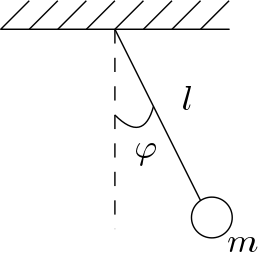
\includegraphics[height=4cm]{matoscill.png}
\qquad \qquad \qquad
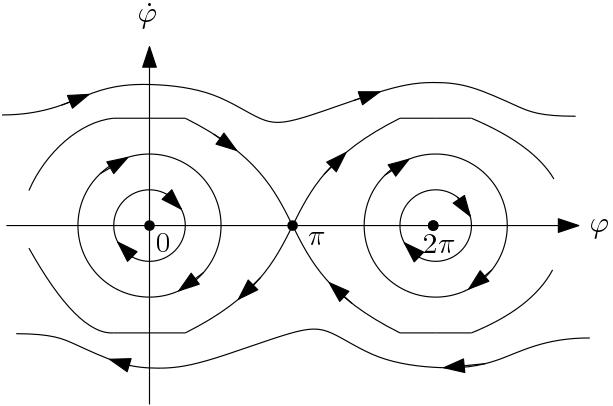
\includegraphics[height=5cm]{phaseportrait.png}
\end{figure}
\begin{flalign*}
& 1) h < - mgl \quad \varnothing &\\
& 2) h = - mgl, \quad \varphi = 0, \;\varphi = 2\pi \text{ --- равновесие} &\\
& 3) -mgl < h < mgl \text{ --- колебания} &\\
& 4) h = mgl \text{ --- либо равновесие $\varphi = \pi$, либо движение к $\varphi = \pi$} &\\
& 5) h > mgl \text{ --- вращение} &\\
\end{flalign*}
\end{xmp}

\begin{xmp}[Маятник во вращающейся плоскости]
\begin{flalign*}
& n = 1, q = \varphi &\\
& T = \frac{m}{2} \v v^2 = \frac{m}{2}\left( r^2\dot \varphi^2 + \omega^2r^2\sin^2 \varphi \right) &\\
& \Pi = - mgr\cos \varphi &\\
& L = T - \Pi, \quad \pd{L}{t} = 0 \Rightarrow T_2 \underbrace{- T_0 + \Pi}_{\Pi^*} = const &\\
& \Pi^* = - mgr\cos \varphi - \frac{m}{2} r^2 \omega^2 \sin^2 \varphi &\\
& \pd{ \Pi^*}{\varphi} = mgr\sin \varphi - \frac{1}{2}mr^2\omega^2 \sin 2\varphi = mr\sin \varphi(g - r\omega^2\sin\varphi) = 0 \Leftrightarrow &\\
& \Leftrightarrow 
\left[
\begin{array}{l}
\varphi = 0 \\
\varphi = \pi \\
\varphi = \pm \arccos \frac{g}{r\omega^2} = \varphi_0, \omega^2 > \frac{g}{2} \\
\end{array}
\right. &\\
& \frac{\partial^2 \Pi^*}{\partial \varphi^2} = mgr\cos\varphi - mr^2\omega^2\cos2\varphi &\\
& \left.\frac{\partial^2 \Pi^*}{\partial \varphi^2}\right|_{\varphi = 0} = mr(g - r\omega^2) \gtrless 0 \quad \omega^2 \lessgtr \frac{g}{r} &\\
& \left.\frac{\partial^2 \Pi^*}{\partial \varphi^2}\right|_{\varphi = \pi} = -mr(g + r\omega^2) < 0, &\\
& \left.\frac{\partial^2 \Pi^*}{\partial \varphi^2}\right|_{\varphi = \varphi_0} = mgr\frac{g}{r \omega^2} - mr^2\omega^2 \left(2 \frac{g^2}{r^2\omega^4} - 1\right) = mr\omega^2\left( r - \frac{g^2}{2\omega^4} \right) < 0&\\
\end{flalign*}
\begin{figure}[H]
\centering
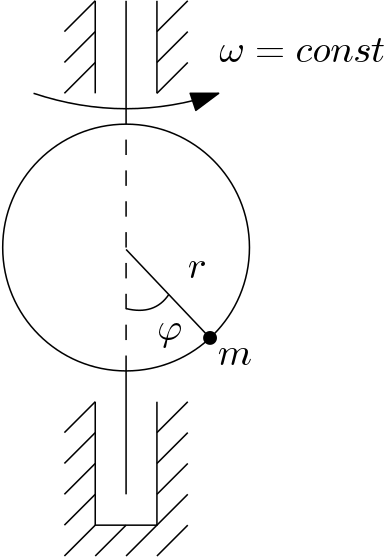
\includegraphics[height=5cm]{rotatingosc.png}
\qquad \qquad \qquad
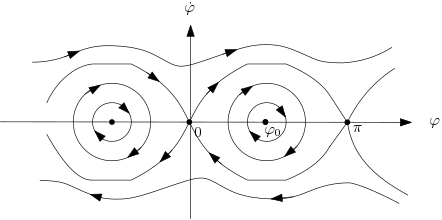
\includegraphics[height=4cm]{otherphaseportrait.png}
\end{figure}
\end{xmp}
  \lline{14.02.2018} \subsection{Элементы теории устойчивости}
\begin{equation}
\label{stable}
\dv x = f(\v x), \, \v x \in \R^n, \, \v f \in C^1: \R^n \rightarrow \R \quad \v x(t) = \v x(t, \v x(0)) \text{ --- начальные условия.}
\end{equation}\

\begin{df}
$ \v x = \v x_0 $ --- положение равновесия \eqref{stable}, если $\v f(\v x_0) = 0$ ($\v x(t, \v x_0 \equiv \v x_0$) $\v x_0 = 0$ без ограничения общности. 
\end{df}

\begin{df}
Равновесие \eqref{stable} устойчиво по Ляпунову, если для любого $\varepsilon > 0$ существует $\delta > 0 $, что любое решение с начальными условиями в $\delta$-окрестности равновесия существует при всех $t > 0$ и находится в $\varepsilon$-окрестности.
\[
	\forall \varepsilon > 0 \ \exists \delta > 0 \ \abs{\v x(0)} < \delta \Rightarrow \abs{\v x(t)} < \varepsilon, \ \forall t > 0.
\]
\end{df}

\begin{df}
$\v x = 0$ --- неустойчивое, если
\[
	\exists \varepsilon > 0 \ \forall \delta > 0 \ \exists \v x(0), t_1 > 0: \abs{x_0} < \delta \ \abs{\v x(t_1, \v x_0)} > \varepsilon
\]
\end{df}

\begin{df}
$\v x = 0$ --- устойчиво асимптотически, если
\begin{enumerate}
\item $\v x = 0$ --- устойчиво,
\item $\lim\limits_{t \rightarrow +\infty} \v x(t, \v x(0)) = 0$. 
\end{enumerate}
\end{df}

\subsection{Прямой метод Ляпунова}
\begin{fl*}
& V(x) &\\
& \dot V = \pd{V}{\v x} \dv x = \pd{V}{\v x} \v f &\\
\end{fl*}

\begin{df}
$\dot V$ --- производная функции $V$ по времени вдоль решения \eqref{stable}.
\end{df}

\begin{teo}[Ляпунова (об устойчивости)]
Если существует гладкая функция $V(x)$ определенная в $\varepsilon$-окрестности равновесия $x = 0$ системы \eqref{stable}, удовлетворяющая следующим условиям:
\begin{enumerate}
\item 
\[
	V(0) = 0, \ \forall x \in U_\varepsilon \setminus \{ 0 \},
\]
\item
\[
	\dot v \leqslant 0 \ \forall \v x \in U_\varepsilon,
\]
\end{enumerate}
то $x = 0$ --- устойчиво по Ляпунову.
\end{teo} 
\begin{proof}
\begin{fl*}
& 1) \forall \varepsilon > 0, \ \exists \sigma = \min V(\v x), \abs{ \v x } = \varepsilon &\\
& 2) V \in C^1 \Rightarrow \exists \delta: V(\v x) < \sigma \ \forall \v x : \abs{\v x} < \delta &\\
& 3) \forall \v x_0: \ \abs{\v x_0} < \delta \ V(\v x(t)) < \sigma \Rightarrow \abs{\v x_0(t)} < \varepsilon \quad (\v x_0(t) = \v x(t, \v x_0)) &\\
\end{fl*}
\end{proof}

\begin{ntc}
\begin{fl*}
& 1) v(0) = 0, v(\v x) > 0 \ \forall \v x \in U_\varepsilon \setminus \{0\} \Rightarrow \text{ $V$ --- положительно определенная функция в 0} &\\
& 2) v(0) = 0, v(\v x) < 0 \ \forall \v x \in U_\varepsilon \setminus \{0\} \Rightarrow \text{ $V$ --- отрицательно определенная функция в 0} &\\
& 3) v(0) = 0, v(\v x) \geqslant (\leqslant) \: 0 \ \forall \v x \in U_\varepsilon \setminus \{0\} \Rightarrow \text{ $V$ --- знакопостоянная функция в 0} &\\
\end{fl*}
\end{ntc}

\begin{xmp}~\\
$V(x_1, x_2) = x_1^2 + x_2^2$ --- положительно определена в $x_1 = x_2 = 0$ \\
$V(x_1, x_2) = x_1^2$ --- не является положительно определенной в $x_1 = x_2 = 0$
\end{xmp}

\begin{ntc}
Если в условии теоремы Ляпунова в условии $2)$ поставить строгое неравенство, устойчивость станет асимптотической.
\end{ntc}

\begin{teo}{Барбашина-Красовского}
Если $\exists V(x) \in C^1 : U_\varepsilon \rightarrow \R$, то
\begin{enumerate}
\item 
\[
	V(0) = 0 \ V(\v x) > 0 \ \forall \v x \in U_\varepsilon \setminus \{ 0 \},
\]
\item
\[
	\dot v \leqslant 0 \  \forall \v x \in U_\varepsilon,
\]
\item множество $\{\v x : \dot v (\v x) = 0\}$ не содержит целиком решения системы \eqref{stable}, кроме равновесия $\v x = 0 \Rightarrow \v x = 0$ --- установившееся асимптотически.
\end{enumerate}
\end{teo}

\begin{ntc}
Если $\dot V < 0$, то $\{ x: \dot V = 0 \} = \{ 0 \}$.
\end{ntc}

\begin{proof}
Пусть $\v x = 0$ установившееся, но не асимптотическое, т.е. 
\begin{fl*}
& I)\  \exists \v x_0(t) \ \abs{\v x_0 (t)} < \varepsilon, \ \v x_0 \not \rightarrow 0 \text{, т.е.} &\\
& \exists \delta, \{t_k\}, \ t_{k + 1} > t_k \ \delta < \abs{\v x_0(t_k)} < \varepsilon &\\
& II)\ \exists \{k_s\} \  \v x_s = \v x_0(t_{k_s}) \xrightarrow{s \rightarrow +\infty} \v x_* &\\
& \abs{\v x_s} > \delta \Rightarrow \abs{\v x_*} > \frac{\delta}{2} &\\
& III)\ V(\v x_0(t)) &\\
& 1),\; 2) \Rightarrow \exists V = \lim_{t \rightarrow + \infty} V(x_0(t)) &\\
& v \in C^1 \Rightarrow v = V(\v x_*) &\\
\end{fl*}
\begin{fl}
\label{triplesec}
& \boxed{\forall t \ V(\v x_0(t)) \geqslant v} &\\
\end{fl}
\begin{fl*}
& IV)\ \text{Рассмотрим} \v x_s(t) = \v x(t, \v x_s) = \v x_0(t + t_{k_s}, \v x_0) &\\
& V)\ \v x_*(t) = \v x(t, \v x_*) &\\
& v(\v x_*) = v, \ 2),\; 3) \Rightarrow \exists t^*: \underbrace{V(\v x_*(t_*))}_{v_*} < v &\\
& VI)\ v \text{ --- непрерывная б.т. } \v x_*(t_*) &\\
& \forall \varepsilon_1 > 0 \ \exists \delta_1 > 0 \ \forall x \ \abs{\v x - \v x_*(t_*)} < \delta_1 \Rightarrow \abs{V(\v x) - V(x_*(t_*))} < \varepsilon_1 &\\
& \text{Решения \eqref{stable} непрерывно и зависит от начальных условий ($t < \infty$)} &\\
& \forall \varepsilon_2 > 0 \ \exists \delta_2 > 0 \ \forall x \ \abs{\v x - \v x_*(t_*)} < \delta_2 \Rightarrow \abs{\v x(t_*) - x_*(t_*)} < \varepsilon_2 &\\
& \forall \varepsilon_3 > 0 \ \exists s: \abs{\v x_s - x_*} < \varepsilon_3 \forall s > S &\\
& \varepsilon_1 = v - v_* > 0 \rightarrow S: \ \abs{V(\v x_s(t_*)) - \underbrace{V(\v x_*(t_*))}_{v_*}} < v - v_* &\\
& V(\v x_s(t_*)) - v_* < v - v_* \text{ --- противоречие с \eqref{triplesec}}
\end{fl*}
\end{proof}

\begin{teo}[Красовского]
$\exists V \in C^1: U_\varepsilon \rightarrow \R$ и область $\Omega$:
\begin{enumerate}
\item $V(0) = 0,\  V(\v x) > 0\  \forall \v x \in U_\varepsilon \cap \Omega$ \\
$\v x = 0 \in \partial \Omega, V(\v x) = 0 \ \forall \v x \in \partial \Omega$
\item $\dot v \leqslant 0 \ \forall \v x \in U_\varepsilon \cap \Omega$
\item $\{ \v x: \dot v = 0 \} \Rightarrow \v x = 0$ --- неустойчивое.
\end{enumerate}
\end{teo}
\begin{proof}
\begin{flalign*}
& \exists \v x = 0 \text{ --- устойчивое, т.е. } &\\
& \forall \varepsilon > 0 \exists \delta > 0: \abs{\v x_0} < \delta \Rightarrow \abs{\v x_0(t)} < \varepsilon &\\
& 1), 2) \Rightarrow \exists \delta: \abs{\v x_0(t)} > 0 \Rightarrow \exists\{ x_s \} \rightarrow \v x_*, &\\
& V(\v x_s(t)) \leqslant V(\v x_*) = v &\\
& \v x_*(t),\  3) \Rightarrow \exists t_* > 0: (\v x_*(t_*)) > v \text {--- противоречие как в предыдущей теореме} &\\
\end{flalign*}
\end{proof}

\begin{ntc}
$\dot v > 0$ --- теорема Четаева.
\end{ntc}

\begin{xmp}[Волчок Эйлера]
MISSING
\end{xmp}
  \lline{21.02.2018} \subsection{I-й метод Ляпунова}
\begin{equation}
\label{onec}
\dv x = A \v x \quad A = const \quad \det(A - \lambda E) = 0
\end{equation}

\begin{ass}
Если все корни характеристического многочлена линейной системы \eqref{onec} имеет отрицательные вещественные части, то равновесие $\v x = 0$ этой системы асимптотически устойчиво по Ляпунову:
\[
	\re \lambda_i < 0 \; \forall i \Rightarrow \v x = 0 \text{ --- асимптотически устойчиво.}
\]
\end{ass}
\begin{proof}
\begin{flalign*}
& 1)\; \lambda_i \in \R. \; \lambda_i \neq \lambda_j \; \forall i \neq j &\\
& \v x = \sum_{i = 1}^n C_i\v u_i e^{\lambda_it}, \; c_i = const, \; \v u_i = const &\\
& \v x = 0 \text{ --- устойчиво асимптотически (по определению).} &\\
& 1)\; \lambda_1 = \lambda_2, \; \v u_i \neq \v u_2 \text{ --- устойчивость.} &\\
& 2)\; \lambda_0 \text{ --- корень кратности } s: &\\
& \v x = + \ldots + (C_1\v u_1 + \ldots + C_s\v u_s t^{s - 1})e^{-\lambda_0t} \Rightarrow \v x = 0 \text{ --- устойчиво асимптотически (по определению).} &\\
& 3)\; \lambda_k = \alpha_k \pm i\beta_k \text{ --- кратность 1} &\\
& \v x = + \ldots + (C_1 \v u_1 e^{(\alpha_k + i\beta_k)t} + C_2 \v u_2 e^{(\alpha_k + i\beta_k)t}) = + \ldots + e^{\alpha_kt}(C_1'\v u\sin\beta_kt + C_2' \v u \cos\beta_kt) \Rightarrow \text{устойчивость.}
\end{flalign*}
\end{proof}

\begin{ass}
Если существует хотя бы 1 корень характеристического уравнения с положительной вещественной частью, то равновесие $\v x = 0$ неустойчиво:
\[
	\exists \lambda_k > 0 \Rightarrow \v x = 0 \text{ --- неустойчиво.}
\]
\end{ass}
\begin{proof}
Аналогично.
\end{proof}

\begin{flalign*}
& (*)\; \dv x = f(\v x) \quad \v f(0) = 0 &\\
& \dv x = A\v x + O(\norm{\v x}^2) \quad A = \pd{\v f}{\v x}\vert_{\v x = 0} = const &\\
& \dv x = A \v x \text{ --- линеаризованная система} &\\
& \det(A - \lambda E) = 0 &\\
\end{flalign*}

\begin{teo}[Ляпунова об устойчивости по первому приближению]
Если все корни характеристического уравнения \emph{линеаризованной системы} имеют отрицательные вещественные части, то равновесие $\v x = 0$ \emph{нелинейной системы} асимптотически устойчиво, если же существует корень с положительной вещественной частью, то равновесие неустойчиво.
\end{teo}
\begin{ntc}[Критический случай]
Если нет $\lambda_k > 0$ $\lambda_k = 0$\footnote{Нечетко записано}, то про систему ничего нельзя сказать
\end{ntc}

\begin{xmp}
\begin{flalign*}
&C > A > B&\\
&\begin{cases}
A\dot p = (B - C)qr \\
B\dot q = (C - A)r(p' + \omega) \\
C\dot r = (A - B)q(p' + \omega) \\
\end{cases} 
\qquad \text{ Линеаризованная: } 
\begin{cases}
A\dot p = 0 \\
B\dot q = (C - A)r\omega \\
C\dot r = (A - B)q\omega \\
\end{cases}&\\
& \v x = (p', q, r)^T &\\
& \mathbb{A} = 
\left(\begin{matrix}
0 & 0 & 0 \\
0 & 0 & \frac{C - A}{B}\omega \\
0 & \frac{A - B}{C}\omega & 0 \\
\end{matrix}\right) &\\
& \det(\mathbb A - \lambda E) = \lambda\left( \lambda^2 - \frac{(C - A)(A - B)}{BC}\omega^2 \right) = 0 \Leftrightarrow
\left[
\begin{array}{l}
\lambda = 0 \\
\lambda = \pm \sqrt{\frac{(C - A)(A - B)}{BC}} \omega 
\end{array}
\right. \Rightarrow &\\
& \Rightarrow \text{ $\v x = 0$ --- неустойчиво, т.к. $\exists \lambda > 0$} &\\
\end{flalign*}
(Из прошлой лекции (не успели) $V = BCqr$)
\end{xmp}

\begin{xmp}
\begin{flalign*}
& \begin{cases}
\dot x = y + \alpha x^3 \\
\dot y = - x \\
\end{cases}
(**) &\\
& \text{Линеаризованная система: }
\begin{cases}
\dot x = y \\
\dot y = -x \\
\end{cases} \qquad
\lambda = \pm i 
\begin{cases}
x = C_1\sin t + C_2\cos t \\
y = C_1\cos t - C_2\sin t \\
\end{cases} &\\
& V = \frac{x^2 + y^2}{2} \quad \dot V = (\dot x x + \dot y y)\vert_{(**)} = \alpha x^4 &\\
& \underline{\alpha < 0} : V(0) = 0 \quad V(x) > 0 \;\forall \v x \neq 0 \quad \dot V \leqslant 0 \;\forall \v x \in U_\varepsilon &\\
& \dot V = 0 \Leftrightarrow x \equiv 0 \quad (**)\vert_{x \equiv 0} \quad \begin{cases}
0 = y + 0 \\
\dot y = 0 \\
\end{cases} \Leftrightarrow y = 0 \Rightarrow \v x = 0 \text{ --- устойчиво асимптотически.} &\\
\end{flalign*}
\begin{figure}[H]
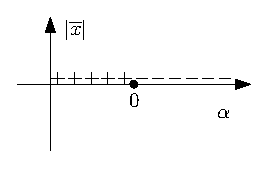
\includegraphics{3_1.eps}
\caption*{Бифуркационная диаграмма}
\end{figure}
\begin{flalign*}
& \underline{\alpha} > 0: \Omega = U_{\varepsilon \setminus \{0\}} &\\
& V(\v x) > 0, \quad \dot V(\v x) > 0, \quad \forall \v x \in \Omega &\\
& V(0) = 0, \quad V(\v x) = 0, \quad \forall \v x \in \partial \Omega (x = 0) &\\
& \Rightarrow \text{ неустойчивость, т.к. } \dot V = 0 \Rightarrow x = y = 0 &\\
\end{flalign*}
\end{xmp}

\begin{equation}
\label{threesta}
\det (A - \lambda E) = 0 \qquad a_0 \lambda^n + a_1\lambda^{n - 1} + \ldots + a_n = 0, \quad a_0 > 0
\end{equation}

\begin{xmp}
\begin{flalign*}
& n = 2: a_0\lambda^2 + a_1\lambda + a_2 = 0,\; a_0 > 0 &\\
& a_1^2 \geqslant 4a_0a_2 : \lambda_1 + \lambda_2 = - \frac{a_1}{a_0}, \; \lambda_1\lambda_2 = \frac{a_2}{a_0} &\\
& \re \lambda_{1, 2} = \lambda_{1, 2} < 0 \Leftrightarrow a_2 >0, a_1 > 0 &\\
& a_1^2 < 4a_0a_2: \re \lambda_{1, 2} = -\frac{a_1}{a_0} < 0 \Rightarrow a_2 >0, a_1 > 0 &\\
& \re \lambda_{1, 2} < 0 \Leftrightarrow a_i > 0, \; i = 1, 2 &\\
\end{flalign*}
\end{xmp}

\begin{ass}[Необходимое условие устойчивости]
Если все корни \eqref{threesta} при $n > 2$ имеют отрицательные вещественные части, то коэффициенты этого уравнения положительны:
\[
	\re \lambda_i < 0 \Rightarrow a_i > 0 \quad i = 1, \ldots, n
\]
\end{ass}
\begin{proof}
\begin{flalign*}
& \lambda_1, \ldots, \lambda_k \text{ --- действительные корни, } \lambda_i < 0,\; i = 1, \ldots, k &\\
& \lambda = \alpha_i \pm \beta_i i \quad j = 1, \ldots, m &\\
& f(\lambda) = a_0(\lambda - \lambda_1) \cdot \ldots \cdot (\lambda - \lambda_k)(\lambda - \alpha_1 - \beta_1 i) \cdot \ldots \cdot (\lambda - \alpha_1 + \beta_1 i)\cdot \ldots &\\ 
& = a_0(\lambda + \abs{\lambda_1}) \cdot \ldots \cdot (\lambda + \abs{\lambda_k})((\lambda + \abs{\alpha_1})^2 + \beta_1^2)\cdot \ldots = a_0\lambda^n + a_1\lambda^{n - 1} + \ldots + a_n \quad a_i > 0 \quad i = 1, \ldots, n &\\
\end{flalign*}
\end{proof}

\begin{xmp}
\[
	f(\lambda) = (\lambda^2 + 1)(\lambda + 1) = \lambda^3 + \lambda^2 + \lambda + 1 
\]
\end{xmp}

\begin{teo}[Критерий Рауса-Гурвица][б/д] 
$\forall i \re \lambda_i < 0 \Leftrightarrow$ все главные диагональные миноры определены положительно
\[
	\Delta = \left(
	\begin{matrix}
	a_1 & a_3 & a_5 & \ldots & 0 \\
	a_0 & a_2 & a_4 & \ldots & 0 \\
	0 & a_1 & a_3 & \ldots & 0 \\
	\vdots & & & \ddots & \vdots \\
	0 & 0 & 0 & \ldots & a_n \\
	\end{matrix}
	\right),
	\qquad \Delta_i > 0
\]
\end{teo}

\begin{ntc}
\[
	\Delta_n = a_n \Delta_{n - 1}
\]
\end{ntc}

\subsection{Равновесие натуральных систем}
Натуральная система:
\begin{gather*}
	L = \frac{1}{2}(A(\v q)\dv q, \dv q) - \Pi(\v q) \\
	\dv x = f(\v x), \; \v x = (q_1, \ldots, q_n, \dot q_1, \ldots, \dot q_n) \\
	\v q = \v q_0 \text{ --- равновесие}, \; \left(\left. \pd{\Pi}{q}\right|_{\v q = \v q_0} = 0 \right)
\end{gather*}
\begin{df}
$\v q = \v q_0$ --- установившееся равновесие положение равновесия натуральной системы, если
\[
	\forall \varepsilon > 0 \; \exists \delta > 0 \; \norm{\v q(0) - \v q_0} + \norm{\dv q(0)} < \delta \Rightarrow \norm{\v q(t) - \v q_0} + \norm{\dv q(t)} < \varepsilon \; \forall t > 0.
\]
\end{df}

\begin{teo}[Лагранжа-Дирихле]
Точка строго локального минимума потенциальной энергии натуральной системы является устойчивым по Ляпунову положением равновесия этой системы:
\end{teo}
\begin{proof}
\begin{flalign*}
& V = T + \Pi(\v q) - \Pi(\v q_0) &\\
& 1)\; V \vert_{\v q = \v q_0,\; \dv q = 0} = 0, V(\v q, \dv q) = \frac{1}{2}(A\dv q, \dv q) + \Pi(\v q) - \Pi(\v q_0) > 0 \quad (A \text { --- положительно определенная}) &\\
& \forall \v q, \dv q: \delta > \norm{\dv q} + \norm {\v q - \v q_0} > 0 &\\
& 2)\; \dot V = 0 \Rightarrow \dv q = 0, \v q = \v q_0 \text{ --- устойчиво.}
\end{flalign*}
\end{proof}

\begin{xmp}
\begin{flalign*}
& \Pi = \begin{cases}
0,\; q = 0 \\
e^{ -\frac{1}{\abs{q}}} \cdot \cos \frac{1}{\abs{q}},\; q \neq 0 
\end{cases} &\\
& 1)\; q = 0 \text{ --- положение равновесия} &\\
& 2)\; q = 0 \neq \min \Pi &\\
& 3)\; T + \Pi = h = const &\\
& \Pi \leqslant h, \; x = 0 \text{ --- устойчиво по Ляпунову (по опр.)} &\\
\end{flalign*}
\begin{figure}[H]
	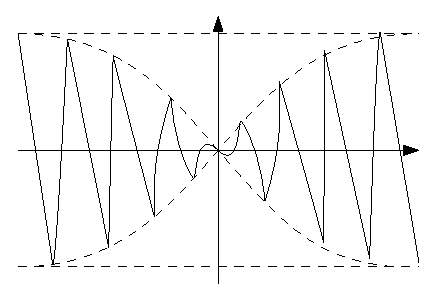
\includegraphics{3_2.eps}
\end{figure}
\end{xmp}
\begin{flalign*}
& \Pi(\v q) = \Pi(\v q_0) + \Pi^{(1)}(\v q) + \Pi^{(2)}(\v q) + \ldots + \Pi^{(m)}(\v q) &\\
& \Pi^{(1)} = \left.\pd{\Pi}{\v q}\right|_{\v q = \v q_0}(\v q - \v q_0) = 0 &\\
& \Pi^{(m)} \text{ --- первая нетривиальная форма } \Pi
\end{flalign*}

  \lline{28.02.2018} \begin{flalign*}
& \v q = 0 \text{ --- положение равновесия} &\\
& T = \frac{1}{2}(A(q)\dv q, \dv q) \quad \Pi = \Pi(0) + \left( \left.\pd{\Pi}{\v q}\right|_{\v q = 0}, \v q \right) + \frac{1}{2}\left(\left.\pd{^2 \Pi}{\v q^2}\right|_{\v q = 0}, \v q \right) + \ldots = \Pi^{(0)} + \Pi^{(1)} + \Pi^{(2)} + \ldots &\\
& \Pi^{(0)} = \Pi(0) = 0, \; \Pi^{(1)} = \left( \left.\pd{\Pi}{\v q}\right|_{\v q = 0}, \v q \right) = 0 &\\
& \Pi^{(m)} \text{ --- первая нетривиальная форма } \Pi &\\
\end{flalign*}

\begin{xmp}
\begin{enumerate}
\item $\Pi(x, y) = \frac{x^4 + y^4}{2}, \quad x = y = 0 \text{ --- устойчивое положение равновесия.}$
\item \begin{flalign*}
& T = \frac{\dot x^2 + \dot y^2}{2} \quad \Pi(x, y) = \frac{x^2}{2} \quad \Pi^{(2)} = \frac{x^2}{2} &\\
& \frac{d}{dt} \pd{T}{\dot x} - \pd{T}{x} + \pd{\Pi}{x} = \ddot x + x = 0 &\\
& \frac{d}{dt} \pd{T}{\dot y} - \pd{T}{y} + \pd{\Pi}{y} = \ddot y = 0 \qquad y = ct + c_1&\\
& x = y = 0 \text{ --- неустойчивое положение равновесия.} &\\
\end{flalign*}
\end{enumerate}
\end{xmp}

\begin{teo}
Если $\Pi$ не имеет даже нестрогого минимума в окрестности некоторого положения равновесия натуральной системы, то равновесие неустойчиво.
\end{teo}

\begin{teo}
\begin{flalign*}
& \underline{m = 2, n = 1}: T = \frac{1}{2}a(q)q^2, \; a(q) > 0 &\\
& b = \left.\pd{^2 \Pi}{q^2} \right|_{q = 0} < 0 &\\
& L = \frac{1}{2}a(q)\dot q^2 - \frac{1}{2}bq^2 + O_3(q) &\\
& 0 = \frac{d}{dt}\pd{L}{\dot q} - \pd{L}{q} = a(q)\ddot q + a'_q \dot q^2 - \frac{1}{2}a'_q \cdot \dot q^2 + bq + O_2(q) = &\\
& = a(q)\cdot \ddot q + bq + O_2(q, \dot q) &\\
&
\begin{cases}
\frac{d}{dt}q = \dot q \\
\frac{d}{dt}\dot q = - \frac{bq - O_2(q, \dot q)}{a(0) + O_1(q)} = -\frac{bq}{a(0)} + \cancel{O_2(q, \dot q)} \\
\end{cases} &\\
& \v x = (q, \dot q)^T, \; \dv x = A\v x &\\
& A = \left( \begin{matrix}
0 & 1 \\
- \frac{b}{a(0)} & 0 \\
\end{matrix} \right) &\\
& \det(A - \lambda E) = \lambda^2 + \frac{b}{a(0)} = 0 \Leftrightarrow \lambda^2 = - \frac{b}{a(0)} > 0 &\\
& \lambda = \pm \sqrt{-\frac{b}{a(0)}} &\\
& \re \lambda_+ > 0 \Rightarrow q = 0 \text{ --- неустойчивое положение равновесия.}
\end{flalign*}
\end{teo}

\begin{ntc}
\begin{flalign*}
& L = \underbrace{\frac{1}{2}a(t)q^2 - \frac{1}{2}bq^2}_{L^*} + O_3(q, \dot q) &\\
& C = \left.\pd{^2 \Pi}{q^2}\right|_{q = 0} &\\
& C \text{ --- положительно определена} \Rightarrow q = 0 \text{ --- устойчиво} &\\
& \det C = 0 \text{ --- } ? &\\
& \exists \Delta_i < 0 &\\
\end{flalign*}
\end{ntc}

\subsection{Влияние гироскопических и диссипативных сил на устойчивость равновесия}
\begin{flalign*}
& \frac{d}{dt}\pd{L}{\dv q} - \pd{L}{\v q} = Q^* &\\
& L = \frac{1}{2}(A(q)\dv q, \dv q) - \Pi(q) &\\
& \dot E = (\v Q^*, \dv q)  \qquad E = T + P &\\
\end{flalign*}

\begin{itemize}
\item Если $(\v Q^*,\; \dv q) = 0$, то $\v Q^*$ --- гироскопическая.
\item Если $(\v Q^*,\; \dv q) \leqslant 0$, то $\v Q^*$ --- диссипативная.
\item Если $(\v Q^*,\; \dv q) < 0$, то $\v Q^*$ обладает полной диссипацией.
\end{itemize}

\begin{teo}[Кельвина-Четаева 1]
Если $q = 0$ --- точка строгого локального минимума $\Pi$ натуральной системы, то даже при добавлении в систему гироскопических и (или) диссипативных сил, она является устойчивым положением равновесия $A$. Если при этом диссипативные силы обладают полной диссипацией, то это равновесие устойчиво асимптотически.
\end{teo}
\begin{proof}
\begin{flalign*}
& V(\v q, \dv q) = T + \Pi(\v q) - \Pi(q) &\\
& q = 0 \text{ --- строгий локальный минимум } \Pi(q) \Rightarrow V(0, 0) = 0,\; V(\v q, \dv q) > 0 \quad \forall \v q, \dv q \; 0 < \norm{q}^2 + \norm{\dv q}^2 < \varepsilon &\\
& a) \dot V = (\v Q^*, \dv q) \leqslant 0 \Rightarrow q = 0 \text{ --- устойчиво по теореме Ляпунова} &\\
& b) \dot V = 0 \Leftrightarrow \dv q = 0 \Leftrightarrow q = 0 \Rightarrow q = 0 \text{ --- устойчиво асимптотически по т. Барабашина-Красовского} &\\
\end{flalign*}
\end{proof}

\begin{teo}[Кельвина-Четаева 2]
Если в изолированном положении равновесия $\Pi$ не имеет даже нестрогого минимума, а силы обладают полной диссипацией, то равновесие неустойчиво (вне зависимости от направления гироскопических сил).
\end{teo}
\begin{proof}
\begin{flalign*}
& V(\v q, \dv q) = T + \Pi(\v q) - \Pi(0) &\\
& q = 0 \text{ --- ...} \Rightarrow \Omega: \Pi(\v q) < \Pi(0) \; \forall q \in \Omega &\\
& \qquad \qquad \qquad \qquad \Pi(q) = \Pi(0) \; \forall q \in \partial \Omega, \; q = 0 \in \partial Q &\\
& V < 0, \dot V < 0 \quad \forall \{\v q, \dv q\} \in \Omega' = \{ \v q, \dv q : q \in \Omega, \dv q = 0 \} &\\
& \dot V = 0 \Leftrightarrow \v q = 0 &\\
& \Rightarrow q = 0 \text{ --- неустойчиво по теореме Красовского.}
\end{flalign*}
\end{proof}

\begin{xmp}
\begin{flalign*}
	& \ddot x = 0,\; x = 0 \text{ --- неустойчиво.} &\\
	& \ddot x = -k\dot x,\; k > 0 &\\
	& \lambda^2 + k\lambda = 0 \Rightarrow \begin{cases}
		\lambda = 0 \\
		\lambda = -k < 0 \\
	\end{cases}&\\
	& \ddot x = 0,\; x = 0 \text{ --- неустойчиво.} &\\
	& \ddot x = -k\dot x,\; k > 0 &\\
	& \lambda^2 + k\lambda = 0 \Rightarrow \begin{cases}
		\lambda = 0 \\
		\lambda = -k < 0 \\
	\end{cases}&\\
	& x = 0 \text{ --- устойчиво.} &\\
\end{flalign*}
\end{xmp}
\begin{xmp}[Гироскопическая стабильность]
	\begin{flalign*}
		& T = \frac{\dot x^2 + \dot y^2}{2} \qquad \Pi = -\frac{x^2 + y^2}{2} \qquad \v Q^* = 2 \dot y \v e_x - 2 \dot x \v e_y &\\
		& (\v Q^*,\dv q) = 2 \dot y\dot x - 2 \dot x\dot y = 0 &\\
		& \begin{cases}
			\ddot x - x = 2 \dot y \\
			\ddot y - y = -2 \dot x \\
		\end{cases} \qquad \left( \dv x = A\v x,\ \det(A - \lambda E) = 0 \right) &\\
		& A\ddot{\v x} + B\dv x + C \v x = 0 &\\
		& \det(A\lambda^2 + B\lambda + C) = 0 &\\
		& A = \left( \begin{matrix}
			1 & 0 \\
			0 & 1 \\
		\end{matrix} \right) \qquad B = \left( \begin{matrix}
			0 & -2 \\
			2 & 0 \\
		\end{matrix} \right) \qquad C = \left( \begin{matrix}
			-1 & 0 \\
			0 & -1 \\
		\end{matrix} \right) &\\
		& \det(A\lambda^2 + B\lambda + C) = \begin{vmatrix}
			\lambda^2 - 1 & -2\lambda \\
			2\lambda & \lambda^2 - 1 \\
		\end{vmatrix} = \lambda^4 - 2\lambda^2 + 1 + 2 ^2\lambda^2 &\\
		& \left[ \begin{array}{l}
			\lambda^2 = -2 \\
			\lambda^2 = -\frac{1}{2} \\
		\end{array} \right. \qquad \begin{array}{l}
			\lambda = \pm \sqrt 2 i \\
			\lambda = \pm \frac{\sqrt 2}{2}i \\
		\end{array} &\\
		& x = y = 0 \text{ --- устойчивое.} &\\
	\end{flalign*}
\end{xmp}

\subsection{Элементы теории бифуркации}
\begin{flalign*}
& \dv x = \v f(\v x, \alpha),\; \v x \in \R^{n},\; \alpha \in \R^n &\\
& \text{Кривые равновесий } \v x = \v x(\alpha): \v f(\v x(\alpha), \alpha) = 0 &\\
& \text{Точка бифуркации } (\v x_*, \alpha_*): \left.\pd{\v f}{\v x} \right|_{\v x = \v x^*(\alpha_*), \; \alpha = \alpha_*} = 0
\end{flalign*}

\begin{figure}[H]
	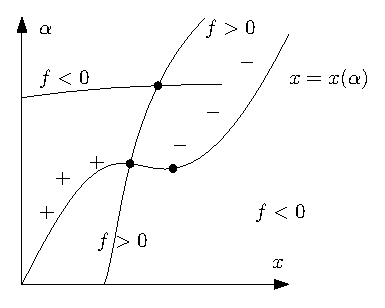
\includegraphics{4_1.eps}
\end{figure}
\begin{flalign*}
	& \underline{n = 1}\quad \dot x = f(x,\;\alpha) &\\
	& \dot x = f'_x(x - x(\alpha)) + O_2(x - x(\alpha)) &\\
	& \lambda = f_x' > 0 \Rightarrow x = x(\alpha) \text{ --- неустойчиво.} &\\
	& \lambda = f_x' < 0 \Rightarrow x = x(\alpha) \text{ --- устойчиво.} &\\
	& \lambda = f_x' = 0 \Rightarrow \text{бифуркация.} &\\
\end{flalign*}
\subsubsection*{Основные типы бифуркаций.}
\begin{figure}[H]
	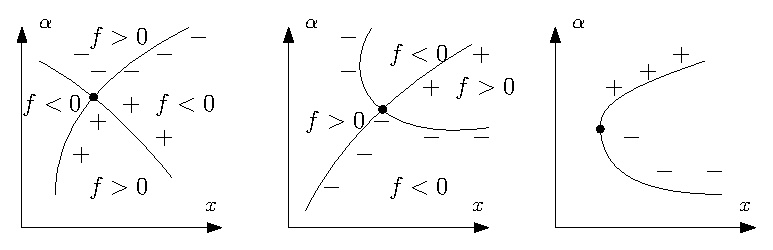
\includegraphics{4_2.eps}
	\caption*{1) Смена устойчивости, 2) вилка, 3) складка.}
\end{figure}
\begin{flalign*}
	& \frac{d}{dt}\pd{L}{\dv q} - \pd{L}{\v q} = 0 \qquad L = \frac{1}{2}\left( A(q)\dv q,\; \dv q \right) - \Pi(\v q,\; \alpha) &\\
	& \text{Кривая равновесия } \left.\pd{\Pi}{\v q}\right|_{\v q = \v q(\alpha)} = 0 &\\
	& \text{Точка бифуркации } \det\left( \left.\pd{^2 \Pi}{\v q^2}\right|_{\v q_* = \v q(\alpha_*), \alpha = \alpha_*} \right) = 0 &\\
	& \underline{n = 1}\quad a\ddot q + bq = 0,\; b = \pd{^2 \Gamma}{q^2} &\\
	& a\lambda^2 + b = 0 &\\
	& \lambda^2 = -\frac{b}{a} &\\
	& 1) b > 0 \quad \lambda = \pm\sqrt{\frac{b}{a}}i \text{ --- устойчиво.} &\\
	& 2) b < 0 \quad \lambda = \pm \sqrt{-\frac{b}{a}} \text{ --- неустойчиво.} &\\
	& \text{Равновесия: } \left[\begin{array}{l}
		\varphi = 0 \\
		\varphi = \pi \\
		\varphi = \pm \arccos \frac{g}{\omega^2r} \\
	\end{array}\right.
\end{flalign*}
\begin{figure}[H]
	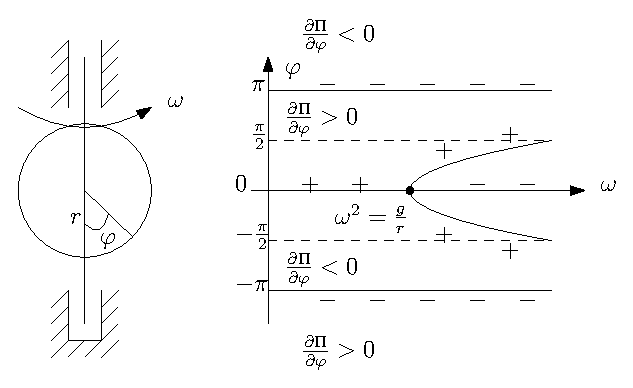
\includegraphics{4_3.eps}
\end{figure}
  \lline{07.03.2018} \begin{xmp}[Бифуркация Андронова-Копфа]
	\begin{flalign*}
		& \begin{cases}
			\dot x = \alpha x - y - x(x^2 + y^2) \\
			\dot y = x + \alpha y - y(x^2 + y^2) \\
		\end{cases} &\\
		& x = y = 0 \text{ равновесие. Откинем квадратичную часть.} &\\
		& \det(A - \lambda E) = \begin{vmatrix}
			\alpha - \lambda & - 1 \\
			1 & \alpha - \lambda \\
		\end{vmatrix} = \lambda^2 - 2\alpha\lambda + \alpha^2 + 1 &\\
		& \alpha < 0 \Rightarrow x = y = 0 \text{ --- устойчиво.} &\\
		& \alpha > 0 \Rightarrow x = y = 0 \text{ --- неустойчиво.} &\\
	\end{flalign*}
	\begin{figure}[H]
		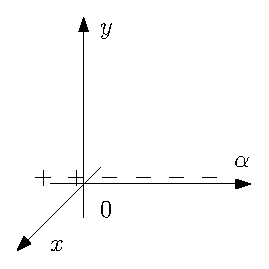
\includegraphics{5_1.eps}
	\end{figure}
	\begin{flalign*}
		& x = r\cos\varphi,\; y = r\sin\varphi &\\
		& \begin{cases}
			\dot r\cos\varphi - r\dot\varphi\sin\varphi = \alpha r \cos\varphi - r\sin\varphi - r\cos\varphi\cdot r^2 & | \cdot \cos\varphi\\
			\dot r\sin\varphi + r\dot\varphi\cos\varphi = r\cos\varphi + \alpha r\sin\varphi - r\sin\varphi\cdot r^2 & | \cdot \sin\varphi\\
		\end{cases} &\\
		& \begin{cases}
			\dot r = \alpha r - r^3  & (1)\\
			\dot \varphi = 1 \\
		\end{cases} &\\
		& r = 0,\; r = \pm\sqrt{\alpha} \text{ --- равносильные уравнению } (1). &\\
	\end{flalign*}
	\begin{figure}[H]
		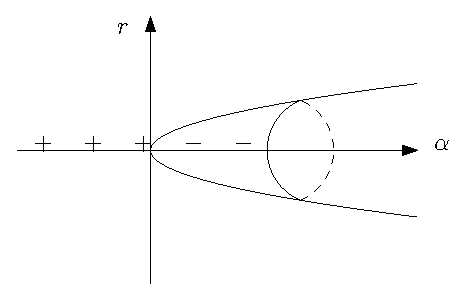
\includegraphics{5_2.eps}
	\end{figure}
	\begin{flalign*}
		& \delta r = r - \sqrt{\alpha} &\\
		& \delta \dot r = \dot r,\; r = \delta r + \sqrt{\alpha} &\\
		& (1) \Leftrightarrow \delta \dot r - (\delta r + \sqrt{\alpha})(-\delta r)(\delta r + 2\sqrt \alpha) = -2\alpha\delta r + O_2(\delta r) &\\
		& \delta r = o(r \pm \sqrt \alpha) \text{ --- устойчивое.}
	\end{flalign*}
	\begin{figure}[H]
		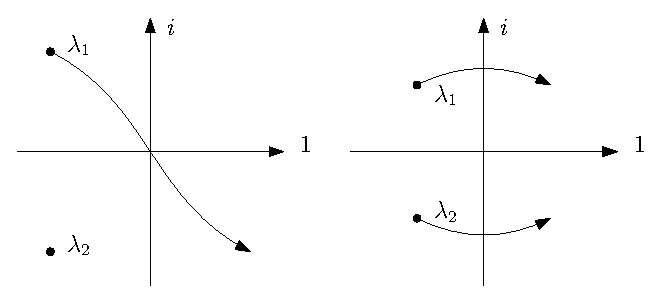
\includegraphics{5_3.eps}
		\caption*{1) Дивергенция. 2) Флаттер.}
	\end{figure}
\end{xmp}

\subsection{Малые Колебания}
\begin{flalign*}
& T = \frac{1}{2}(\Phi(\v q)\dv q, \dv q), \; \Pi(\v q), \; \v q = 0 \text{ --- положение равновесия} &\\
& \Pi(\v q) = \underbrace{\Pi(0)}_0 + \left( \left.\pd{\Pi}{\v q}\right|_{\v q = 0}, \v q \right) + \frac{1}{2}\left( \left.\pd{^2 \Pi}{\v q^2}\right|_{\v q = 0}, \v q \right) + O_3(\v q) &\\
& \left. \pd{^2 \Pi}{\v q^2} \right|_{\v q = 0} = c = const, \quad C = C^T &\\
& T = \frac{1}{2}\left(\left(\Phi(0) + O(\norm{\v q})\right)\dv q, \dv q\right) = \frac{1}{2}(A \dv q, \dv q) + O_3(\v q, \dv q) &\\
& A = \Phi(0) = const, \; A = A^T &\\
& L = \tilde L + O_3(\v q,\dv q),\; \tilde L = \frac{1}{2}(A\dv q, \dv q) - \frac{1}{2}(C\v q, \v q) &\\
& \pd{\tilde L}{\dv q} = \frac{1}{2}\underbrace{(A\dv q + A^T \dv q)}_{\text{Из 3 семестра}} = A \dv q, \quad \frac{\tilde L}{\v q} = -C\v q \text{ --- аналогично} &\\
& \frac{d}{dt}\pd{\tilde L}{\dv q} - \pd{\tilde L}{\v q} = 0 \Leftrightarrow \boxed{A\ddot{\v q} + C\v q = 0} &\\
& \text{$A$ положительно определена } \xrightarrow{\text{Из линейной алгебры}} \exists \v e_1, \ldots, \v e_n: \: A \rightarrow E, C \rightarrow k &\\
& \v q = \sum \xi_i \v e_i = u \v \xi, \tilde L = \frac{1}{2}(E \dv \xi, \dv \xi) - \frac{1}{2}(k \v \xi, \v \xi), &\\
& k = \diag(k_1, \ldots, k_n) &\\
& \text{Уравнения Лагранжа:} &\\
& \ddot{\v \xi} + k\v \xi = 0 \Rightarrow \begin{cases}
\ddot{\xi}_1 + k_1\xi_1 = 0 \\
\vdots \\
\ddot{\xi}_n + k_n\xi_n = 0 \\
\end{cases} &\\
& \text{Пусть } k_i = \omega_i^2 > 0 &\\
& k \text{ и } C \text{ --- положительно определены, } \v q = 0 (\v \xi = 0) \text{ --- устойчиво по теореме Лагранжа-Дирихле} &\\
& \ddot \xi_i + k_i \xi_i = 0 \quad \lambda^2 + k_i, \quad \lambda^2 + \omega_i^2 = 0 \quad \lambda = \pm \omega_i i &\\
& \xi_i = C_{1i} \sin \omega_i t + C_{2i}\cos \omega_i t = \alpha_i\sin(\omega_i t + \varphi_i) &\\
& \v q = \sum_{i = 1}^n \alpha_i \v e_i \sin(\omega_i t + \varphi_i)
\end{flalign*}

\begin{ass}
\begin{flalign*}
& \det (A \omega^2 - C) = 0 &\\
& \begin{cases}
A(\omega_i^2 - C) e_i = 0 \\
(A \v e_i, \v e_i) = 1 \\
\end{cases},
i = 1, \ldots, n
\end{flalign*}
\end{ass}
\begin{proof}
\begin{flalign*}
& 2\tilde \Pi = (C\v q, \v q) = (CU\v \xi, U\v \xi) = (U^TCU\v \xi, \v \xi) = (k\v \xi, \xi) \Leftrightarrow k = U^TCU &\\
& 2\tilde T = (A\dv q, \dv q) = (U^TAU\v \xi, \v \xi) = (E\dv \xi, \dv \xi) \Leftrightarrow &\\
& \Leftrightarrow E = U^TAU (\Leftrightarrow (A\v e_i, \v e_j) = \delta_{ij}) &\\
& k - k_iE = \diag(k_1 - k_i, \ldots, k_{i - 1} - k_i, 0, \ldots) &\\
& \det(k - k_iE) = 0 \Leftrightarrow \det(U^TCU - k_iU^TAU) = 0 \Leftrightarrow &\\
& \Leftrightarrow \det U^T \det(C - Ak_i)\det U = 0 \leftarrow\xrightarrow{\det U \neq 0} \det(Ak_i - C) = 0, \det(A \omega_i^2 - C) = 0 &\\
& 2) (k - k_iE)(0, \ldots, 0, \underbrace{1}_i, 0, \ldots)^T &\\
& (U^TC - k_iU^TA)\underbrace{U(0, \ldots, 0, 1, 0, \ldots, 0)^T}_{\v e_i} \qquad C\v q = \sum \v e_i\xi_i &\\
& U^T(C - \omega_i^2 A)\v e_i = 0 \Leftrightarrow (A\omega_i - C)\v e_i = 0 &\\
\end{flalign*}
\end{proof}

\begin{df}
$\det(A\omega^2 - C) = 0$ --- вековое уравнение (уравнение частот). $\omega_i$ --- частоты малых колебаний (собственные частоты).
\end{df}

\begin{cor}
Частоты малых колебаний не зависят от выбора обобщенных координат.
\end{cor}

\begin{df}
Если $(A\omega_i^2 - C)\v U_i = 0$, то $\v U_i$ --- амплитудный вектор, соответствующий частоте $\omega_i$.
\end{df}

\begin{ntc}
$\v U_i = \beta_i \v e_i,\; \beta_i = const$
\end{ntc}

\begin{flalign*}
& \v q = \sum_{i = 1}^n \tilde \alpha_i \v U_i \sin(\omega_i t + \varphi_i) &\\
\end{flalign*}

\begin{cor}
\begin{enumerate}
\item Ортогональность
\[
	(A\v U_i, \v U_j) = 0, \; i \neq j
\]
\item Линейная независимость
\begin{gather*}
C_1U_1 + \ldots + C_nU_n = 0 \\
0 + \ldots + (A\v U_i, C_i \v U_i) + \ldots + 0 = 0 \Leftrightarrow C: (A\v U_i, \v U_i) = 0 \Leftrightarrow C_i = 0 \\
(A\v U, \v U) = 0 \Leftrightarrow \v U = 0
\end{gather*}
\end{enumerate}
\end{cor}

\begin{ntc}
$\tilde \alpha, \varphi$ --- определяются начальными условиями.
\end{ntc}

\begin{flalign*}
I.\;\; &\tilde \alpha_i = 0, \quad \forall i \neq m: \v q = \tilde \alpha_m \v U_m \sin(\omega_m t + \varphi_m) &\\
& \text{главные (нормальные) колебания} &\\
Ia.\;& \text{Кратные частоты } \omega_1 = \omega_2 = \omega &\\
& k = \diag(\omega_1^2, \omega_2^2, \ldots) &\\
& \begin{cases}
\ddot \xi_1 + \omega^2 \xi_1 = 0 \\
\ddot \xi_2 + \omega^2 \xi_2 = 0
\end{cases} &\\
& (A\omega^2 - C)\v U = 0 &\\
& U = C_1\v U_1 + C_2\v U_2 &\\
II.\;& \exists k_m = 0 &\\
& \ddot \xi_m = 0,\; \xi_m = C_1t + C_2 &\\
III.& \exists k_m < 0, \v q = 0 (\xi = 0) \text{ --- неустойчиво.} &\\
& \ddot \xi_m + k_m\xi_m = 0 &\\
& \lambda^2 = -k_m > 0 &\\
& \lambda = \pm \sqrt{-k_m}
\end{flalign*}

\begin{teo}
Если $\Pi^{(2)}_{(0)}$ не имеет даже нестрогий минимум, то $\v q = 0$ неустойчиво.
\end{teo}
\begin{proof}
\begin{flalign*}
& \underline{n = 1} \text{ уже доказано} &\\
& \underline{n > 1} \quad \v q \rightarrow \v \xi &\\
& \begin{cases}
\ddot \xi_1 + k_1\xi_1 = 0 \\
\vdots \\
\ddot \xi_n + k_n\xi_n = 0 \\
\end{cases} &\\
& \exists k_m < 0: \ddot \xi_m + k_m \xi_m = 0 \text{ ---||--- } &\\
\end{flalign*}
\end{proof}

\subsection{Вынужденные колебания в линейных системах}
\begin{flalign*}
& \ddot x + \omega_0^2x = f\cos\omega t &\\
& x = x_{\text{одн}} + x\text{ч} &\\
& x_{\text{одн}} = C_1 \sin \omega_0 t + C_2\cos \omega_0t &\\
& 1)\; \omega \neq \omega_0: x\text{ч} = \alpha\sin \omega t + \beta\cos \omega t \quad /\; \omega_0^2 &\\
& \qquad \dot x\text{ч} = \alpha\omega\cos\omega t - \beta\omega\sin\omega t \quad /\; 0 &\\
& \qquad \ddot x\text{ч} = -\alpha\omega^2\sin\omega t - \beta\omega^2\cos\omega t \quad /\; 1 &\\
& \begin{cases}
\alpha \omega_0^2 - \alpha \omega^2 = 0 \\
\beta \omega_0^2 - \beta \omega^2 = f \\
\end{cases}
\Rightarrow
\begin{cases}
\alpha = 0 \\
\beta = \frac{f}{\omega_0^2 - \omega^2}
\end{cases} &\\
& x = C_1\sin \omega_0t + C_2\cos \omega_0 t + \frac{f}{\omega_0^2 - \omega^2}\cos\omega t
\end{flalign*}
\begin{figure}[H]
	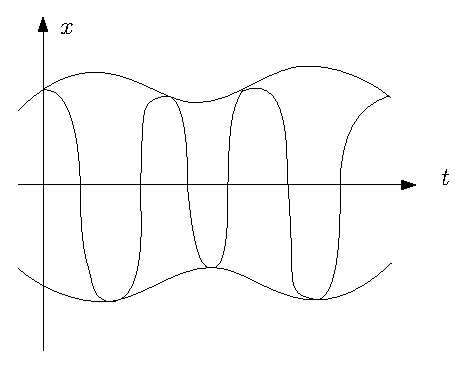
\includegraphics{5_4.eps}
	\caption*{Биения.}
\end{figure}
\begin{flalign*}
& 2)\; \omega = \omega_0 \quad x\text{ч} = \alpha t \sin \omega_0 t &\\
& \qquad \dot x\text{ч} = \alpha \sin\omega_0t + \alpha \omega_0t\cos \omega_0t &\\
& \qquad \ddot x\text{ч} = \alpha \omega_0 \cos \omega_0 t - \alpha \omega_0 t \sin \omega_0 t \Rightarrow 2\alpha \omega_0 = f \Rightarrow \alpha = \frac{f}{2\omega_0} &\\
& x = C_1 \sin \omega_0t + C_2\cos \omega_0t + \frac{f}{2\omega_0}t \sin \omega_0t
\end{flalign*}
\begin{figure}[H]
	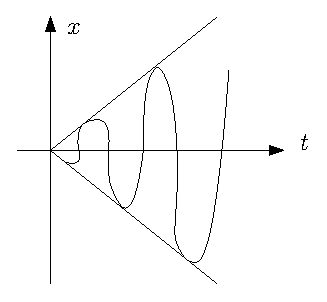
\includegraphics{5_5.eps}
	\caption*{Резонанс.}
\end{figure}
\begin{flalign*}
& A\ddot{\v q} + C \v q = \v Q, \quad \v Q = \v F \cos \omega t &\\
& \v q = U \v \xi, \quad A \rightarrow E, \; C \rightarrow K &\\
& (\v Q, \delta \v q) = (\v Q, U\delta \v \xi) = (U^T\v Q, \delta \v \xi) = (\v Q \delta \v \xi) &\\
& \tilde Q = U^T \tilde Q &\\
\end{flalign*}
  \lline{14.03.2018} \begin{flalign*}
& A\ddot{\v q} + C \v q = \v Q = \ddot \xi_i + \omega^2 \xi_i = \tilde Q_i, \quad i = 1, \ldots, n &\\
& 1)\; \v Q = \v F\cos \omega t, \quad Q_i = \mu_i \cos \omega t \qquad \tilde Q = U^T\v F &\\
& \ddot \xi_i + \omega_i^2 \xi_i = \mu_i\cos \omega t &\\
& \left[ 
\begin{array}{ll}
\omega \neq \omega_i,\; \forall i = 1, \ldots, n & \xi_i = \alpha_i \cos (\omega_it + \beta_i) + \frac{\mu_i}{\omega_i^2 - \omega^2} \cos \omega t \\
\omega = \omega_k,\; \mu_k = 0, & \xi_k = \alpha_k \cos(\omega_kt + \beta_k) + \frac{\mu_k}{2\omega} \sin \omega t
\end{array}
\right. &\\
& 2)\; \v Q \text{ периодично по $t$: } (\v Q(t + T) = \v Q(t), \forall t \in (0; +\infty)) &\\
& \v Q(t) = \v F\left(a_0 + \sum_{k = 1}^{+\infty} A_k \cos\left(\frac{2\pi k t}{T} + Q_k \right)\right) &\\
& \v q = \v q_{\text{одн}} + \sum_{k = 0}^{+\infty}\v q_r^{(k)} &\\
& \omega_i = \frac{2\pi k}{T}
\end{flalign*}

\begin{xmp}
\begin{flalign*}
& \ddot x + k \dot x + \omega_0^2 x = f \sin \omega t, \; k > 0 &\\
& x = 0 \text{ --- равновесие (установившееся асимптотически) свободной системы} &\\
& \lim_{x \rightarrow +\infty} x_\text{одн} = 0 &\\
& x_r = R\sin(\omega t + \varphi) &\\
& \dot x_r = R\omega\sin(\omega t + \varphi) &\\
& \ddot x_r = - R\omega^2\sin(\omega t + \varphi) &\\
& R(\omega_0^2 - \omega^2)\sin(\omega t + \varphi) + KR\omega\cos(\omega t + \varphi) = f\sin \omega t &\\
& R = \frac{f}{\sqrt{(\omega^2 - \omega^2)^2 + k^2 \omega^2}}, \quad \varphi = - \arctg \frac{k\omega}{\omega_0^2 - \omega^2} &\\
& ((\omega_0^2 - \omega^2) + k^2\omega^2)'_\omega = -2(\omega_0^2 - \omega^2)\cdot 2\omega + 2k^2\omega = 0 \Leftrightarrow 
\left[\begin{array}{l}
\omega = 0 \\ 
\omega^2 = \omega_0^2 - \frac{k^2}{2} \\
\end{array}\right. &\\
\end{flalign*}
РИСУНКИ чего-то
\end{xmp}

\begin{flalign*}
& \frac{d}{dt}\pd{l}{\dot q} - \pd{L}{\v q} = \v Q^* + \v Q(t) &\\
& \v Q^* = B \dv q,\; B = const &\\
& \v q = 0 \text{ --- устойчиво асимптотически} &\\
& \det(A\lambda^2 + B\lambda + C) = 0 \Leftrightarrow \re \lambda_i < 0, \; i = 1, \ldots, n &\\
& P(\lambda) = A\lambda^2 + B\lambda + C &\\
& \v Q(t) = \v F \sin \omega t \Rightarrow \v Q(t) = \v Fe^{i\omega t} &\\
& \v q = \v q_r = \v h e^{i\omega t} \quad \dv q = \v h i \omega e^{i \omega t} \quad \ddot{\v q} = \v h(i\omega)^2 e^{i\omega t} &\\
& D(i\omega) \v h = \v F \quad \det D(i\omega) \neq 0 &\\
& \v h = [D(i\omega)]^{-1} \v F = W(i\omega) \v F, \; W(i\omega) = (w_{kj}), \; k,j = 1, \ldots, n &\\
& w_{kj} = |w_{kj}|e^{i\arg \omega_{kj}} = R_{kj}e^{i\varphi_{kj}} &\\
& R_{kj} = |w_{kj}| \qquad \v q = W(i\omega)\v F e^{i\omega t} &\\
& \varphi_{kj} = \arg \omega_{kj} \qquad \sum_{j = 1}^n w_{kj}F_j e^{i\omega t} = \sum R_{kj} F_j e^{i(\omega t + \varphi_{kj})}
\end{flalign*}
РИСУНОК чего-то

\section{Гамильтонова механика}
\subsection{Преобразования Лежандра}
Рассмотрим $X(\v x): \; \R^n \rightarrow \R, \; X(\v x) \in C$.
\begin{flalign*}
& \det \pd{^2 X}{x^2} \neq 0 &\\
& \v y = \v f(\v x) = \pd{X}{x} &\\
& \Rightarrow \v x = \v f^{-1}(\v y) = \v x(\v y) &\\
& Y(\v y) = ((\v x, \v y) - X(\v x)) \vert_{\v x = \v x(\v y)} &\\
\end{flalign*}

\begin{df}
$Y(\v y)$ --- преобразование Лежандра функции $X(\v x)$ по переменной $\v x$.
\end{df}
Свойства преобразований Лежандра\footnote{Возможно, тут чего-то не хватает}:
\begin{enumerate}
\item Инвалютивность.
\begin{flalign*}
& X,\v x \rightarrow Y, \; \v y \rightarrow X, \v x &\\
& \pd{Y}{y_i} = x_i + \left( \pd{\v x}{y_i}, \v y \right) - \left( \pd{X}{\v x}, \pd{\v x}{y_i} \right) = &\\
& x_i + \left(\underbrace{\v y - \pd{X}{\v x}}_0, \pd{\v x}{y}\right) = x_i, \; i = 1, \ldots, n \Rightarrow &\\
& \Rightarrow \v x = \pd{Y}{\v y}
\end{flalign*}
\item \begin{flalign*}
& \pd{^2}{\v y^2} = \pd{\v x}{\v y} = \left( \pd{\v y}{\v x} \right)^{-1} = \left( \pd{^2 X}{\v x^2} \right)^{-1} &\\
& \det \pd{^2 Y}{\v y^2} = \left( \det \pd{^2 X}{\v x^2} \neq 0 \right) &\\
\end{flalign*}
\item \begin{flalign*}
& \v x, X \rightarrow \v y, Y = [(\v x, \v y) - X(\v x)]\vert_{\v x = f'(\v y)} \rightarrow \v z, Z &\\
& \v y = \v f_2(\v z),\; \v z = \v x,\; \v y = f_2^{-1}(\v x),\; f'(f_2^{-1}) = \v x &\\
& Y(\v y)_{\v y = f_2^{-1}(\v x)} = (\v x, \v y \vert_{\v y = f_2^{-1}(\v x)}) - X(\v x) &\\
& X(\v x) = [(\v x, \v y) - Y(\v y)]\vert_{\v y = \v y(x)}
\end{flalign*}
\item \begin{flalign*}
& X = X(\v x, \alpha), \alpha \in \R &\\
& Y = Y(\v y, \alpha) &\\
& \pd{X}{\alpha} = -\pd{Y}{\alpha} &\\
& Y(\v y, \alpha) = ((\v x, \v y(\v x, \alpha)) - X(\v x, \alpha)) \vert_{\v x = \v x(\v y, \alpha)} &\\
& \pd{Y}{\alpha} = \left( \pd{\v x}{\alpha}, \v y \right) - \left( \pd{X}{\v x}, \pd{\v x}{\alpha} \right) - \pd{X}{\alpha} =  &\\
& = \left( \pd{\v x}{\alpha}, \underbrace{\v y - \pd{X}{\v x}}_0 \right) - \pd{X}{\alpha} = - \pd{X}{\alpha}
\end{flalign*}
\end{enumerate}

Повторим это с лагранжианом.
\begin{flalign*}
& L = L(q, \dot q, t)
\end{flalign*}
\begin{df}
$p = \pd{L}{\dot q}$ --- обобщенный импульс.
\end{df}
\begin{flalign*}
& \det \pd{^2 L}{\dot q^2} \neq 0 \Rightarrow \dot q = \dot q(q, p, t) &\\
& H(q, p, t) = [(\dot q, p) - L(q, \dot q, t)]\vert_{\dot q = \dot q(q, p, t)} &\\
\end{flalign*}

\begin{df}
$H$ --- гамильтониан (функция Гамиильтона).
\end{df}
\begin{df}
$(q, p, t)$ --- канонические переменные (параметры Гамильтона).
\end{df}
\begin{teo}
В канонических переменных уравнения движения имеют вид
\[
	\begin{cases}
	\dot q = \pd{H}{p} \\
	\dot p = -\pd{H}{q} \\
	\end{cases}
\]
\end{teo}
\begin{proof}
\begin{flalign*}
& \text{Инвалютивность} \Rightarrow \dot q = \pd{H}{p} &\\
& \dot p = \frac{dp}{dt} = \frac{d}{dt}\pd{L}{\dot q} = \frac{L}{q} = -\pd{H}{q}
\end{flalign*}
\end{proof}

\begin{df}
\begin{flalign*}
& \dv x = \v F(\v x, t) \v x \in \R^{2n} \text{ --- гамильтонова система, если} &\\
& \v x = (q_1, \ldots, q_n, p_1, \ldots, p_n)^T \quad \exists H = H(q, p): &\\
& \v F = \left( \pd{H}{p_1}, \ldots, \pd{H}{p_n}, -\pd{H}{q_1}, \ldots, -\pd{H}{q_n} \right)^T
\end{flalign*}
\end{df}
ПРИМЕР
  \lline{21.03.2018} \subsection{Первый интеграл и понижение порядка в уравнении Гамильтона}
\begin{df}
$q_k$ --- циклическая переменная, если $\pd{H}{q_k} = 0 \left( \pd{L}{q_k} = -\pd{H}{q_k} \right)$.
\end{df}

\begin{ass}
Если $q_k$ --- циклическая координата, то $p_n = const$.
\end{ass}
\begin{proof}
\begin{flalign*}
& \dot p_n = -\pd{H}{q_n} = 0 \Rightarrow p_n = const. &\\
\end{flalign*}
\end{proof}

\begin{ass}
Если $\pd{H}{t} = 0$, то $H = const$.
\end{ass}
\begin{proof}
\begin{flalign*}
& \frac{dH(q, p, t)}{t} = \left( \pd{H}{q}, \dot q \right) + \left( \pd{H}{p}, \dot p \right) + \pd{H}{t} = \pd{H}{t} = 0 \Rightarrow H = const &\\
\end{flalign*}
\end{proof}

\begin{flalign*}
& \pd{H}{q_n} = 0 \Rightarrow p_n = const = \beta &\\
& H = H(q_1, \ldots, q_{n - 1}, p_1, \ldots, p_{n - 1}, \beta, t) &\\
& \tilde q = (q_1, \ldots, q_{n - 1})^T, \quad \tilde p = (p_1, \ldots, p_{n - 1})^T &\\
& H = H(\tilde q, \tilde p, \beta, t) &\\
& \begin{cases}
\dot{\tilde q} = \pd{H(\tilde q, \tilde p, \beta, t)}{\tilde p} \\
\dot{\tilde p} = \pd{H(\tilde q, \tilde p, \beta, t)}{\tilde q} \\
\end{cases}
\end{flalign*}

\begin{ass}
При $\beta = const$ (заданном значении циклического интеграла $\beta$) уравнения движения системы имеют вид
\[
\begin{cases}
\dot{\tilde q} = \pd{H(\tilde q, \tilde p, \beta, t)}{\tilde p} \\
\dot{\tilde p} = \pd{H(\tilde q, \tilde p, \beta, t)}{\tilde q} \\
\end{cases}
\Leftrightarrow
\left.\left(\begin{cases}
\dot q = \pd{H}{p} \\
\dot p = -\pd{H}{q} \\
\end{cases}\right)\right|_{\beta = const}
\]
\end{ass}

\begin{flalign*}
& \begin{cases}
\tilde q = \tilde q (t, c_1, \ldots, c_{2n - 2}, \beta) \\
\tilde p = \tilde p (t, c_1, \ldots, c_{2n - 2}, \beta) \\
\end{cases} (*) &\\
& p_n = \beta = const &\\
& \dot q_n = \left.\left( \pd{H(\tilde q, \tilde p, t, \beta)}{p_n} \right)\right|_{(*)} = f(t, c_1, \ldots, c_{2n - 2}, \beta) &\\
& \frac{dq_n}{dt} = f \Rightarrow q_n = \int\limits_0^t f(\tau, c_1, \ldots, c_{2n - 2}, \beta)d\tau + c_{2n - 1} &\\
\end{flalign*}

\begin{flalign*}
& \pd{H}{t} = 0 \Rightarrow H(q, p) = const = h &\\
& \text{Пусть } \pd{H}{p_n} \neq 0 \Rightarrow p_n = p_n(q_1, \ldots, q_n, p_1, \ldots, p_{n - 1}, h) = -K(\tilde q, \tilde p, \tau, h), &\\
& \text{где } \tilde q = (q_1, \ldots, q_{n - 1})^T, \; \tilde p = (p_1, \ldots, p_{n - 1})^T,\; \tau = q_n 
\end{flalign*}

\begin{df}
$K(\tilde q, \tilde p, \tau, h)$ --- функция Уиттекера.
\end{df}

\begin{ass}
Уравнения Гамильтона на фиксированном уровне интеграла энергии локально эквивалентны уравнениям Уиттекера
\[
	\begin{cases}
	\tilde q' = \pd{K}{\tilde p} \\
	\tilde p' = -\pd{K}{\tilde q} \\
	\end{cases},
	\quad
	\tilde q' = \frac{d\tilde q}{d\tau}, \; \tilde p' = \frac{d\tilde p}{d\tau}.
\]
\end{ass}
\begin{proof}
\begin{flalign*}
& H(\tilde q, \tau, \tilde p, -K) \equiv h &\\
& 0 = \pd{H}{p_i} - \pd{H}{p_n} \cdot \pd{K}{p_i} = \dot q_i - \dot q_n \cdot \pd{K}{p_i} \Rightarrow \frac{\dot q_i}{\dot q_n} = \pd{K}{p_i} \Rightarrow \frac{dq_i}{d\tau} = \pd{K}{p_i}, \quad i = 1, \ldots, n - 1 &\\
& \frac{dH}{dq_i} = 0 = \pd{H}{q_i} - \pd{H}{p_n}\pd{K}{q_i} = - \dot p_i - \dot q_n \pd{K}{q_i} \Rightarrow \frac{\dot p_i}{\dot q_n} = -\pd{K}{q_i} \Rightarrow \frac{dp_i}{d\tau} = -\pd{K}{q_i}, \quad i = 1, \ldots, n - 1 &\\
& \tilde q = \tilde q(\tau, c_1, \ldots, c_{2n - 2}) &\\
& \tilde p = \tilde p(\tau, c_1, \ldots, c_{2n - 2}) &\\ &\\
& p_n = - K(\tilde q(q_m, c_1, \ldots, c_{2n-2}), \tilde p(q_n, c_1, \ldots, c_{2n - 2}), q_n, h) = p_n(q_n, c_1, \ldots, c_{2n - 2}, h) &\\
& \dot q_n = \pd{H}{p_n} = f(q_n, c_1, \ldots, c_{2n - 2}, h) &\\
& \int\limits_0^t\frac{dq_n}{f(q_n, c_1, \ldots, c_{2n-2}, h)} = t + c_{2n - 1} &\\
\end{flalign*}
\end{proof}

\subsection{Скобки Пуассона}
\begin{df}
Скобкой Пуассона двух функций $F(q, p)$ и $G(q, p)$ называется
\[
	\{F, G\} = \left( \pd{F}{q}, \pd{G}{p} \right) - \left( \pd{F}{p}, \pd{G}{q} \right) = \sum_{i = 1}^n \left( \pd{F}{q_i}\pd{G}{p_i} - \pd{F}{p_i}\pd{G}{q_i}\right)
\]	
\end{df}

\begin{enumerate}
\item Линейность
\begin{flalign*}
& \{F, \alpha_1 G_1 + \alpha_2 G_2\} = \alpha_1\{F, G_1\} + \alpha_2\{F, G_2\} &\\
& \alpha_1 = const, \alpha_2 = const &\\
\end{flalign*}
\item Антикоммутативность
\begin{flalign*}
& \{F, G\} = -\{G,F\}
\end{flalign*}
\item Тождество Якоби-Пуассона\footnote{Доказательство не доведено до конца}
\begin{flalign*}
& \{F, \{G, W\}\} + \{G, \{W, F\}\} + \{W, \{F, G\}\} = 0 &\\
& \{F, \{G, W\}\} = \sum_{i = 1}^n \pd{F}{q_i}\pdd{\sum_{j = 1}^n\left(\pd{G}{q_j}\pd{W}{p_j} - \pd{G}{p_j}\pd{W}{q_j}}{p_i}\right) - &\\
& - \sum_{i = 1}^n \pd{F}{p_i}\pdd{\sum_{j = 1}^n\left(\pd{G}{q_j}\pd{W}{p_j} - \pd{G}{p_j}\pd{W}{q_j}}{q_i}\right) = \ldots &\\
\end{flalign*}
\item Правило Лейбница
\begin{flalign*}
& \{F_1F_2, G\} = F_1\{F_2, G\} + F_2\{F_1, G\} &\\
\end{flalign*}
\item $\{\varphi(F_1, \ldots, F_k), G\} = \sum\limits_{i = 1}^k \pd{\varphi}{F_i}\{F_i, G\}$
\item \begin{flalign*}
& F = F(q, p, t), \; G = G(q, p, t) &\\
& \pdd{\{F, G\}}{t} = \left\{\pd{F}{t}, G\right\} + \left\{F, \pd{G}{t}\right\} &\\
& \pdd{\{F, G\}}{q_i} = \left\{\pd{F}{q_i}, G\right\} + \left\{F, \pd{G}{q_i}\right\} &\\
& \pdd{\{F, G\}}{p_i} = \left\{\pd{F}{p_i}, G\right\} + \left\{F, \pd{G}{p_i}\right\} &\\
\end{flalign*}
\end{enumerate}

\begin{xmp}
\begin{flalign*}
& \begin{cases}
\dot q = \pd{H}{p} \\
\dot p = -\pd{H}{q} \\
\end{cases}
\Leftrightarrow
\begin{cases}
\dot q_i = \{q_i, H\} \\
\dot p_i = \{p_i, H\} \\
\end{cases} &\\
\end{flalign*}
\end{xmp}

\begin{ass}
Функция $F(q, p, t)$ --- первый интеграл системы с гамильтонианом $H(q, p, t)$ тогда, и только тогда, когда
\[
	\pd{F}{t} + \{F, H\} = 0.
\]
\end{ass}
\begin{proof}
\begin{flalign*}
& \pd{F}{t} = \left( \pd{F}{q}, \dot q \right) + \left( \pd{F}{p}, \dot p \right) + \pd{F}{t} = \{F, H\} + \pd{F}{t} &\\
\end{flalign*}
\end{proof}
\begin{ntc}
\[
	\frac{dF}{dt} = 0 \Leftrightarrow \pd{F}{t} + \{F, H\} = 0
\]
\end{ntc}
\begin{teo}[Якоби-Пуассона]
Скобка Пуассона двух первых интегралов в уравнении Гамильтона также является первым интегралом этих уравнений.
\end{teo}
\begin{proof}
Пусть $F_1$ и $F_2$ --- первые интегралы системы с гамильтонианом $H$.
\begin{flalign*}
& \pd{F_1}{t} + \{F_1, H\} = 0, \; \pd{F_2}{t} + \{F_2, H\} = 0 &\\
& \pdd{\{F_1, F_2\}}{t} + \{\{F_1, F_2\}, H\} = \left\{ \pd{F_1}{t}, F_2 \right\} + \left\{ F_1, \pd{F_2}{t} \right\} - \{H, \{F_1, F_2\}\} = &\\
& = \{F_2, \{F_1, H\}\} + \{F_1, \{H, F_2\} \} + \{H, \{F_1, F_2\}\} = 0 \Leftrightarrow \{F_1, F_2\} \text{ --- первый интеграл.} &\\
\end{flalign*}
\end{proof}

\begin{flalign*}
& L = \frac{1}{2}(A\dot q, \dot q) + (B, \dot q) - \Pi(q, t) &\\
& H = \frac{1}{2}(A^{-1}(p - B), (p - B)) + \Pi(1, t) = \underbrace{\frac{1}{2}(A^{-1}p, p)}_{H_2} - \underbrace{(A^{-1}p, B)}_{H_1} + \underbrace{\Pi(q, t) + \frac{1}{2}(A^{-1}B, B)}_{H_0}
\end{flalign*}

\begin{ass}
$H = H(q_1, \ldots, q_{n - 1}, p_1, \ldots, p_{n - 1}, f(q_n, p_n), t) \Rightarrow f(q_n, p_n) = const = \alpha$
\end{ass}
\begin{df}
$q_n, p_n$ --- отделяющиеся переменные
\end{df}
\begin{proof}
\begin{flalign*}
& \pd{f}{t} + \{f, H\} = 0 + \pd{f}{q_n} \pd{H}{p_n} - \pd{f}{p_n}\pd{H}{q_n} = \pd{f}{q_n}\pd{H}{f}\pd{f}{p_n} - \pd{f}{p_n} \pd{H}{f} \pd{f}{q_n} = 0 &\\
\end{flalign*}
\end{proof}
  \lline{28.03.2018} \begin{flalign*}
& L = L(q, \dot q, t) &\\
& \gamma = \{q(t), t \in [t_1, t_2]\; q(t_1) = q_1,\; q(t_2) = q_2\} \text{ --- какая-то траектория} &\\
& \Omega = \{q(t) \in C^2, t \in [t_1, t_2]\; q(t_1) = q_1,\; q(t_2) = q_2\} &\\
& \gamma \in \Omega &\\
\end{flalign*}

\begin{df}
Кривая, соответствующая решению уравнения Лагранжа системы с лагранжианом $L$ называется прямым путем системы. Остальные пути называются окольными.
\end{df}
\begin{ntc}
Прямой путь не единственный.
\end{ntc}
\begin{df}
$S$ --- функционал действия по Гамильтону
\[
	S = S(q(t))_{q(t) \in \Omega} = \int\limits_{t_1}^{t_2} L(q(t), \dot q(t), t) dt.
\]
\end{df}
\begin{df}
Семейство кривых $q^\varepsilon(t) = q(t, \varepsilon)^{t \in [t_1, t_2]}_{\varepsilon \in [-\varepsilon_0, \varepsilon_0]}, \; q^\varepsilon(t) \in \Omega$ --- вариация кривой $q(t)$, если 
\begin{enumerate}
\item $q(t_0) = q(t)\; \forall t \in [t_1, t_2]$,
\item $q(\varepsilon, t_1) = q_1,\; q(\varepsilon, t_2) = q_2,\; \forall \varepsilon \in [-\varepsilon_0, \varepsilon_0]$.
\end{enumerate}
\end{df}
\begin{df}
$\delta S = \left( \frac{d}{d\varepsilon}\vert_{\varepsilon = 0} S(q^\varepsilon(t)) \right)\delta \varepsilon$ --- вариация функционала $S$, соответствующая $q(t)$ при вариации $q^\varepsilon(t)$.
\end{df}

\subsection{Принцип Гамильтона}
\begin{ass}
Вариация функционала действия на некотором пути равный нулю тогда, и только тогда, когда путь прямой.
\[
	\delta S = 0\; \forall q^\varepsilon(t) \Leftrightarrow \left.\left( \pdd{\pd{L}{\dot q}}{t} - \pd{L}{q} \right)\right|_{q = q^\varepsilon(t, 0)}
\]
\end{ass}
\begin{proof}
\begin{flalign*}
& S(q^\varepsilon(t)) = \int\limits_{t_1}^{t_2}L(q^\varepsilon(t), \dot q^\varepsilon(t), t)dt &\\
& \vdots &\
\end{flalign*}
MISSING
\end{proof}
  \lline{04.04.2018} \begin{flalign*}
	&(1)\begin{cases}
		\tilde q = \tilde q(q, t, \alpha) \\
		\tilde t = \tilde t(q, t, \alpha) \\
	\end{cases}
	\qquad
	\det\pd{(\tilde q_1, \ldots, \tilde q_n, \tilde t)}{(q_1, \ldots, q_n, t)} \neq 0
	&\\
	& \tilde q(q, t, 0) = q,\; \tilde t(q, t, 0) = t,\ \tilde L(\tilde q, \tilde q', \tilde t) = L(\tilde q, \tilde q', \tilde t) &\\
	& f = (\eta \cdot p) - \zeta H = const &\\
	& p = \pd{L}{\dot q},\; \eta = \left.\pd{\tilde q}{\alpha}\right|_\alpha = 0,\; H = \left( \pd{L}{\dot q},\; \dot q \right) - L,\; \zeta = \left.\pd{\tilde t}{\alpha}\right|_\alpha = 0 &\\
\end{flalign*}
\begin{proof}
\begin{flalign*}
	& (1) \Rightarrow \begin{cases}
		\tilde q = q + \alpha \eta + O_2(\alpha) \\
		\tilde t = t + \alpha \zeta + O_2(\alpha) \\
	\end{cases} (1') &\\
	& \begin{cases}
		q = \tilde q - \alpha \eta + O_2(\alpha) \\
		t = \tilde t - \alpha \zeta + O_2(\alpha) \\
	\end{cases} &\\
	& \dot q = \frac{dq}{dt} = \frac{d}{dt}(\tilde q - \alpha \eta + O_2(\alpha)) = \frac{d\tilde q}{d\tilde t}\frac{d\tilde t}{dt} - \alpha \dot\eta + O_2(\alpha) = q'(1 + \alpha \dot \zeta) - \alpha \dot \eta + O_2(\alpha) &\\
	& \dot q = \tilde q' + \alpha(\dot \zeta \tilde q' - \dot \eta) + O_2(\alpha) = \tilde q' + \alpha(\zeta \dot q - \dot \eta) + O_2(\alpha) \quad (2) &\\
	& \tilde L(\tilde q, \tilde q', \tilde t) = L(q, \dot q, t)|_{(1'),(2)} \cdot \frac{d t}{d \tilde t} = L(\tilde q - \alpha \eta + O_2,\; \tilde q' + \alpha(\zeta\dot q - \dot \eta) + O_2,\; \tilde t - \alpha \zeta + O_2)\cdot \frac{dt}{d \tilde t} = &\\
	& = \left( L(\tilde q, \tilde q', \tilde t) + \alpha \left[ \left( \pd{L}{q}, -\eta \right) + \left( \pd{L}{\dot q}, \zeta \dot q - \dot \eta \right) + \pd{L}{t}(-\zeta)\right] + O_2\right)(1 - \alpha\dot \zeta + O_2) = &\\
	& = L(\tilde q, \tilde q', \tilde t) + \alpha\left[ -\left( \frac{d}{dt}\pd{L}{\dot q}, \eta \right) - \left( \pd{L}{\dot q}, \dot \eta \right) + \dot \zeta\left( \pd{L}{\dot q}, \dot q \right) - \dot \zeta L - \pd{L}{t}\zeta\right] + O_2 = &\\
	& = L(\tilde q ,\tilde q', \tilde t) + \alpha\left[ -(\dot p, \eta) - (p, \dot \eta) + \dot \zeta H + \pd{H}{t} \zeta\right] + O_2 = &\\
	& L(\tilde q, \tilde q', \tilde t) - \alpha \frac{d}{dt}f + O_2(\alpha) = L(\tilde q, \tilde q', \tilde t) &\\
	& \left.\frac{d}{d\alpha}\right|_{\alpha = 0} \Leftrightarrow \frac{df}{dt} = 0 \Leftrightarrow f = const &\\
\end{flalign*}
\end{proof}

\subsection{Интегральный инвариант}
\begin{figure}[H]
	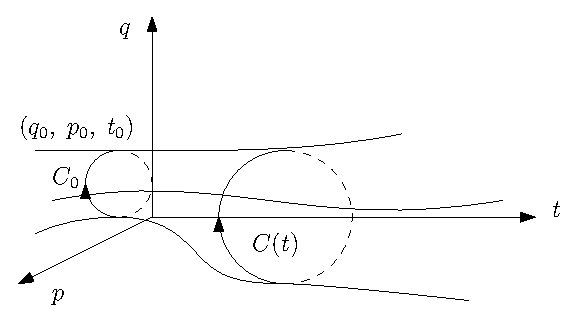
\includegraphics{9_1.eps}
\end{figure}
\begin{flalign*}
	& H = H(q, p, t) &\\
	& (*) \begin{cases}
	\dot q = \pd{H}{p} \\
	\dot p = -\pd{H}{q} \\
	\end{cases} &\\
	& \{q, p, t\} \text{ --- расширенное фазовое пространство.} &\\
	& \begin{cases}
	q = q(t,\; q_0,\; p_0) \\
	p = p(t,\; q_0,\; p_0) \\
	\end{cases}
	\text{ --- прямой путь.} &\\
	& C_0 \rightarrow C(t) &\\
	& I_{\text{п}} = \oint\limits_{C: t = const} \sum\limits_{i = 1}^np_i \delta q_i = \oint(p,\delta q) \text{ --- универсальный интегральный инвариант Пуанкаре.} &\\
\end{flalign*}
\begin{ass}
	Величина $I_{\text{п}}$ сохраняется на всех контурах (изохронах), охватывающих одну и ту же трубку прямых путей системы $(*)$.
\end{ass}
\begin{proof}
	\begin{flalign*}
		& C(t): \begin{cases}
		q = q(\alpha), &\alpha \in [0; 1] \\
		p = p(\alpha), &q(0) = q(1) \\
		t = const, &p(0) = p(1) \\
		\end{cases} &\\
		& \delta q = \pd{q}{\alpha}\delta \alpha &\\
		& \frac{d}{dt} I_{\text{п}} = \oint\limits_C (\dot p, \delta q) + (p, \dot{(\delta q)}) \ovalbox{=} &\\
		& \frac{d}{dt}\delta q = \frac{d}{dt}\left( \pd{q}{\alpha} \right)\delta \alpha = \pdd{\frac{d}{dt}q}{\alpha}\delta \alpha = \delta \dot q &\\ 
		& \ovalbox{=} \oint\limits_C (\dot q, \delta q) + (p, \delta \dot q) = \oint\limits_C \delta(p, \dot q) - \oint\limits_C(\delta p, \dot q) + \oint\limits_C (\dot p, \delta q) \overset{(*)}{=} &\\
		& \overset{(*)}{=} -\oint\limits_C\left( \pd{H}{p}, \delta p \right) + \left( \pd{H}{q}, \delta q \right) = -\oint\limits_C \delta H = 0 \Rightarrow I_{\text{п}} = const
	\end{flalign*}
\end{proof}

\begin{df}
	\[
		I = \oint\big[A(p,\; q,\; t) + (B(q,\; p, \; t), \delta p) + \gamma(q,\; p, \; t)\delta t\big]
	\]
	$I$ --- относительный интегральный инвариант первого порядка системы $(*)$, если $I$ сохраняет свое значение на всех согласованных контурах, охватывающих одну и ту же трубку прямых путей.
\end{df}
\begin{df}
	Контуры согласованы, если если существует такая их параметризация, что каждому значению параметра разных контуров соответствуют точки одного и того же пути.
\end{df}
\begin{figure}[H]
	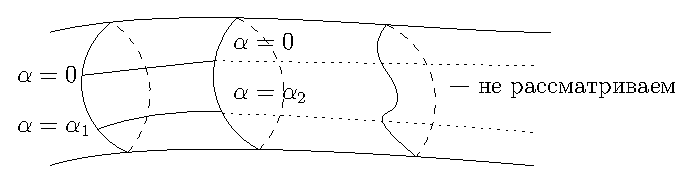
\includegraphics{9_2.eps}
\end{figure}

\begin{teo}[Теорема Ли Хуа-Чжуна]
	\[ 
		I = \oint\limits_{C: t = const} (A(q,\; p,\; t), \delta q) + (B(q,\; p, \; t), \delta p)
	\] 
	--- универсальный (не зависит от гамильтониана) интегральный инвариант системы $(*)$ тогда, и только тогда, когда $I = cI_\text{п},\; c = const$
\end{teo}
\begin{proof}
Для простоты $n = 1$.
\begin{flalign*}
	& \frac{d}{dt} I = \frac{d}{dt} \oint\limits_{C: t = const} A\delta q + B \delta q = \oint\limits_C \dot A\delta q + \dot B \delta p + A\delta \dot q + B \delta\dot p =  \oint\limits_C \delta(A\dot q + B \dot p) - \delta A\dot q - \delta B \dot p + \dot A\delta q + \dot B\delta p = &\\
	& = \oint\limits_C \left( \pd{A}{p}\dot p + \cancel{\pd{A}{q}\dot q} + \pd{A}{t} \right)\delta q - \left( \pd{A}{p} \delta p  + \cancel{\pd{A}{q}\delta q}\right)\dot q + \left(\cancel{\pd{B}{p}\dot p} + \pd{B}{q}\dot q + \pd{B}{t} \right)\delta p - \left( \cancel{\pd{B}{p}\delta p} + \pd{A}{q}\delta q \right)\dot p = &\\
	& = \oint\limits_C -\left( \pd{A}{p} - \pd{B}{q} \right)\pd{H}{p}\delta p + \left( \pd{A}{p} - \pd{B}{q} \right)\left( -\pd{A}{q} \right)\delta q + \pd{A}{t}\delta q + \pd{B}{t}\delta p = &\\
	& = \oint\limits_C \underbrace{\alpha\delta p + \beta\delta q}_{\delta f} = 0 \quad \forall C \Leftrightarrow \pd{f}{q} &\\
	& \begin{cases}
		\pd{f}{q} = -z\pd{H}{q} + \pd{A}{t},\; z = \pd{A}{t} - \pd{B}{q} \\
		\pd{f}{q} = -z \pd{H}{p} + \pd{B}{t} \\
	\end{cases} &\\
	& \frac{\partial^2f}{\partial q \partial p} = \frac{\partial^2 f}{\partial p \partial q} \Leftrightarrow -\pd{z}{p}\pd{H}{q} - \cancel{z\frac{\partial^2H}{\partial p\partial q}} + \frac{\partial^2 A}{\partial p\partial t} = -\pd{z}{p}\pd{H}{q} - \cancel{z\frac{\partial^2H}{\partial q \partial p}} + \frac{\partial^2 B}{\partial q \partial t} &\\
	& -\pd{z}{p}\pd{H}{q} + \pd{z}{q}\pd{H}{p} + \pd{z}{t} = 0 \; \forall H \Leftrightarrow \pd{z}{p} = \pd{z}{q} = \pd{z}{t} = 0 \Leftrightarrow z = c = const &\\
	& \pd{A}{p} - \pd{B}{q} = c &\\
	& \pdd{A - cp}{p} = \pd{B}{q} \Leftrightarrow (A - cp)\delta q + B\delta p = 0 &\\
	& A\delta p + B\delta p = cp\delta q \Rightarrow I = cI_\text{п} &\\
\end{flalign*}
\end{proof}
\begin{df}
	$ I_\text{пк} = \oint (p, \delta q) - H\delta t $ --- интегральный инвариант Пуанкаре-Картана.
\end{df}
\begin{ass}
	$I_\text{пк} = const$.
\end{ass}
\begin{proof}
\begin{figure}[H]
	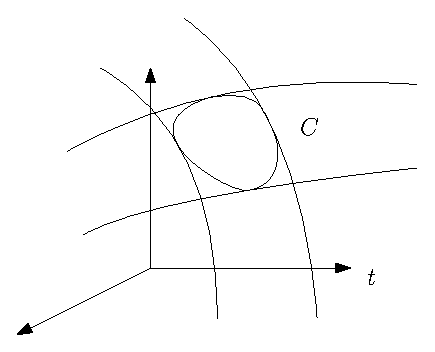
\includegraphics{9_3.eps}
\end{figure}
\begin{flalign*}
	& C:\tau(q, p, t) = const &\\
	& q_{n + 1} = t &\\
	&\begin{cases}
	\dot q = \pd{H}{p} \\
	\dot p = -\pd{H}{q} \\
	\end{cases} &\\
	& q' = \frac{dq}{d\tau} = \frac{dq}{dt}\frac{dt}{d\tau} = \frac{dH}{dp}\eta &\\
	& \eta(q,\; p,\; q_{n + 1}) = \pd{t}{\tau} &\\
	& p' = \frac{dp}{d\tau} = -\pd{H}{q}\eta &\\
	& p_{n + 1} = -H(q,\; p,\; t) \quad q_{n + 1}' = \frac{dt}{d\tau}= \eta &\\
	& \tilde H = \eta(H + p_{n + 1}) \qquad p_{n + 1}' = -\pd{H}{q_{n + 1}}\eta = -\pd{H}{t}\eta &\\
	& \text{Докажем, что $\tilde H$ --- новый гамильтониан.} &\\
	& \pd{\tilde H}{p} = \pd{\eta}{p}(H + p_{n + 1}) + \eta \pd{H}{p} = \eta \pd{H}{p} = q' &\\
	& \pd{\tilde H}{q} = \pd{\eta}{q}(H + p_{n + 1}) + \eta\pd{H}{q} = \eta \pd{H}{q} = - p' &\\
	& \pd{H}{p_{n + 1}} = \eta = q_{n + 1}',\; \pd{\tilde H}{q_{n + 1}} = \pd{\eta}{q_{n + 1}}(H + p_{n + 1}) + \eta\pd{H}{q_{n + 1}} = \frac{dt}{d\tau}\pd{H}{t} = -p_{n + 1}' &\\
	& I = \oint\limits_C(\tilde p, \delta \tilde q) \text{ --- инвариант } \Rightarrow I_\text{пк} = \oint(p, dq) - Hdt &\\
\end{flalign*}
\end{proof}
\begin{flalign*}
	& I = \int\ldots\int dq_1 \ldots dq_n dp_1 \ldots dp_n = V &\\ 
\end{flalign*}
  \lline{11.04.2018} \subsection{Теорема Лиувилля}
\begin{flalign*}
	\dv x = \v f(\v x) \quad (1)
\end{flalign*}
\begin{df}
	\[
		V = \int \ldots \int dx_1 \ldots dx_n 
	\]
	--- фазовый объем.
\end{df}
\begin{df}
	$\v x_0 \rightarrow \v x = \v x(t, \v x_0)$ --- фазовый поток системы $(1)$.
\end{df}
\begin{teo}
	Если $\Div f = 0$, то $V = const$.
\end{teo}
\begin{proof}
	\begin{flalign*}
		& \v x = \v x_0 + t\v f(\v x_0) + O_2(t) &\\
		& V = \int \ldots \int dx_1 \ldots d x_n = \int \ldots \int \abs{\det \pd{\v x}{\v x_0}} dx_{10}\ldots dx_{n0} &\\
		& \det \pd{\v x}{\v x_0} = \det\left( E + t\pd{\v f(\v x_0)}{\v x_0} + O_2 \right) = 1 + t \tr\left( \pd{\v f(\v x_0)}{\v x_0} \right) + O_2 &\\
		& \dot V \vert_{t = 0} = \int \ldots \int \left(0 + \tr \left(\pd{\v f(\v x_0)}{\v x_0}\right) + O_2\right) dx_{10}\ldots dx_{n0} \qquad\qquad \begin{vmatrix}
			1 + t\pd{f_1}{x_{10}} & \overbrace{t\cdot(*)}^{O_2} \\
			t \cdot (-*) & 1 + t\pd{f_2}{x_{20}} \\
		\end{vmatrix} &\\
		& \tr \pd{\v f(\v x_0)}{\v x_0} = 0 \Rightarrow \dot V \vert_{t = 0} = 0 &\\
		& \Div \v f = \sum\pd{f_i}{x_i} = 0 \Rightarrow \dot V \vert_{t = t_*}, \; \forall t_* \Rightarrow V = const &\\
	\end{flalign*}
\end{proof}
\begin{flalign*}
	& \begin{cases}
		\dot q = \pd{H}{p} \\
		\dot p = -\pd{H}{q} \\	
	\end{cases}
	\begin{array}{l}
		\v x = (q_1,\ldots, q_n, p_1,\ldots, p_n)^T \\
		\v f_H = \left( \pd{H}{p_1},\ldots,\pd{H}{p_n}, -\pd{H}{q_1},\ldots,-\pd{H}{q_n} \right) \\
	\end{array}
	&\\
	& \Div \v f_H = \sum_{i = 1}^n \frac{\partial^2H}{\partial q_i \partial p_i} - \sum\limits_{i = 1}^n\frac{\partial^2 H}{\partial p_i\partial q_i} = 0 \Rightarrow V_h = const 
\end{flalign*}
\begin{ntc}
	Такие преобразования фазов. пот. сохраняют $V$.
\end{ntc}

\subsection{Обратные теоремы теории интегральных инвариантов}
\begin{teo}
	Если на любой трубке траектории системы дифференциальных уравнений вида
	\[
		\begin{cases}
			\dot q = Q(q,\; p,\; t) \\
			\dot p = P(q,\; p,\; t)	\\
		\end{cases}
		\quad (*)
	\]
	$I_\text{п} = \oint\limits_{C:t = const} (p, \delta q)$ сохраняется, то данная система гамильтонова.
\end{teo}
\begin{proof}
	\begin{flalign*}
		& \frac{d}{dt}I_\text{п} = \oint\limits_{C: t = const}(\dot p, \delta q) + (p, \delta \dot q) = \oint\limits_{C: t =const} \delta(p, \dot q) - (\delta p, \dot q) + (\dot p, \delta q) \overset{(*)}{=} &\\
		& = \oint\limits_C(P, \delta q) - (Q, \delta p) = 0 \quad \forall C \Leftrightarrow \exists H: (P, \delta q) - (Q, \delta p) = -\delta H = -\left( \pd{H}{p}, \delta p \right) - \left( \pd{H}{q}, \delta q \right) &\\
		& Q = \pd{H}{p},\; P = -\pd{H}{q} &\\
	\end{flalign*}
\end{proof}
\begin{teo}
	Если на любой трубке прямых путей системы $(*)$ $I_\text{пк} = \oint\limits_C (p, dq) - Hdt$, то система гамильтонова с гамильтонианом $H$.
\end{teo}
\begin{proof}
	Возьмем $C_1$, на котором $dt = 0$(изохроны).
	\begin{flalign*}
		& \oint\limits_C(p, dq) - Hdt = \oint\limits_{C_1}(p, dt) \text{ --- инвариант} \Rightarrow \text{ по предыдущей теореме } \exists H(q,\; p,\; t): \begin{cases}
			\dot q = \pd{H^*}{p} \\
			\dot p = -\pd{H^*}{q} \\
		\end{cases}
		\Rightarrow &\\
		& \Rightarrow I_\text{пк}^* = \oint\limits_C(p, dq) - H^*dt = \oint\limits_{C_1}(p, dq) &\\
		& I_\text{пк} - I_\text{пк}^* = \oint\limits_C (H^* - H)dt = 0 \quad \forall C \Leftrightarrow (H^* - H)dt = dF = \left( \pd{F}{q}, dq \right) + \left( \pd{F}{p}, dp \right) + \pd{F}{t}dt &\\
		& \pd{F}{q} = \pd{F}{p} = 0,\; \pd{F}{t} = H^* - H &\\
		& \begin{cases}
			\pd{H}{p} = \pd{H^*}{p} \\
			\pd{H}{q} = \pd{H^*}{q} \\
		\end{cases}
		\Rightarrow
		\text{ система $(*)$ гамильтонова с гамильтонианом $H$.} &\\
	\end{flalign*}
\end{proof}

\subsection{Канонические преобразования}
\begin{flalign*}
	& (1)\begin{cases}
		\dot q = \pd{H}{p} \\
		\dot p = -\pd{H}{q} \\
	\end{cases} \quad
	(2)\begin{cases}
		\tilde q = \tilde q(q,\; p,\; t) \\
		\tilde p = \tilde p(q,\; p,\; t) \\
	\end{cases}
	\Leftrightarrow
	\begin{cases}
		q = q(\tilde q, \tilde p, t) \\
		p = p(\tilde q, \tilde p, t) \\
	\end{cases} &\\
	& H = H(q, p, t) \qquad \det \pd{(\tilde q, \tilde p)}{(q, p)} \neq 0 &\\
	& \dot{\tilde q}\vert_{(1)} = \left.\left( \pd{\tilde q}{q}\dot q + \pd{\tilde q}{p}\dot p + \pd{\tilde q}{t} \right)\right|_{(1)} = Q(\tilde q,\; \tilde p,\; t) \overset{?}{=} \pd{\tilde H}{\tilde p} &\\
	& \dot{\tilde p}\vert_{(1)} = \left.\left( \pd{\tilde p}{p}\dot p + \pd{\tilde p}{p}\dot p + \pd{\tilde p}{t} \right)\right|_{(1)} = P(\tilde q,\; \tilde p,\; t) \overset{?}{=} -\pd{\tilde H}{\tilde q} &\\
\end{flalign*}
\begin{xmp}
\begin{flalign*}
	& H = \frac{p^2 + q^2}{2},\; \begin{cases}
		\tilde q = p^2 \\
		\tilde p = q \\
	\end{cases}
	\quad
	\begin{cases}
		q = \tilde p \\
		p = \pm \sqrt{\tilde q} \\
	\end{cases} &\\
	& \begin{cases}
		\dot q = \pd{H}{p} = p \\
		\dot p = -\pd{H}{q} = -q \\
	\end{cases} \qquad
	\begin{array}{ll}
		\dot{\tilde q} = 2p\dot p = -2pq = \mp2\tilde p \sqrt{\tilde q} & \overset{?}{=} Q = \pd{\tilde H}{\tilde p} \\
		\dot{\tilde p} = p = \pm\sqrt{\tilde q} & \overset{?}{=} P = -\pd{\tilde H}{\tilde q} \\
	\end{array} &\\
	& \pd{Q}{\tilde q} = \pd{P}{\tilde p} \qquad \mp \tilde p \cdot \frac{1}{\sqrt{\tilde q}} \neq 0 \Rightarrow \text{ система не гамильтонова.}
\end{flalign*}
\end{xmp}
\begin{df}
	Неособенное (т.е. обр.) преобразование вида $(2)$ называется каноничным, если оно \emph{любую} гамильтонову систему превращает в гамильтонову систему.
\end{df}
\begin{teo}[Критерий канонического преобразования] 
	Преобразование $(2)$ каноническое $\Leftrightarrow \exists c \neq 0,\; F(q, p, t)$:
	\[
		(\tilde p, d\tilde q) - \tilde Hdt = c((p, dq) - Hdt) - dF
	\]
\end{teo}
\begin{proof}
	\ovalbox{$\Rightarrow$}
	\begin{figure}[H]
		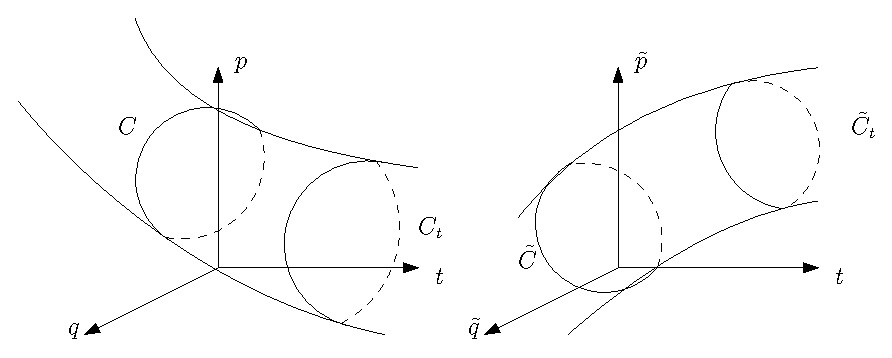
\includegraphics{10_1.eps}
	\end{figure}
	\begin{flalign*}
		& C \xrightarrow{(2)} \tilde C &\\
		& \oint\limits_{\tilde C}(\tilde p, d \tilde q) - \tilde Hdt = \oint\limits_{\tilde C_t: t = const} (\tilde p, \delta \tilde q), \qquad\begin{array}{l}
			\tilde p = \tilde p(q,\; p,\; t) \\
			\tilde q = \tilde q(q,\; p,\; t) \\
		\end{array} &\\
		& \oint\limits_C(\tilde p, d\tilde q) - \tilde Hdt = \oint\limits_{C_t} \left( \tilde p, \pd{\tilde q}{q}\delta q + \pd{\tilde q}{p} \delta p \right) = \oint\limits_{C_t}(A, \delta q) - (B, \delta p) \overset{\text{т. Ли-Хуанчжуна}}{=} &\\
		& = c\oint\limits_{C_t}(p, \delta q) = \left( \oint\limits_C(p, dq) - Hdt \right)c &\\
		& \oint\limits_C\left( (\tilde p, d\tilde q) - \tilde Hdt - c[(p, dq) - Hdt]\right) = 0 \quad \forall C \Leftrightarrow (\tilde p, d\tilde q) - \tilde Hdt = c((p, dq) - Hdt) - dF &\\
	\end{flalign*}
	\ovalbox{$\Leftarrow$} Проинтегрируем равенство
	\begin{flalign*}
		& \oint\limits_C (\tilde p, d\tilde q) - \tilde Hdt = c\oint\limits_C(p, dq) - Hdt - \underbrace{\oint\limits_C df}_{0} = I &\\
		& \oint\limits_{\tilde C} (\tilde p, d\tilde q) - \tilde Hdt = \oint\limits_{C} (p, dq) - Hdt \text{ --- инвариант, т.к. $I$ --- инвариант.} &\\
		& \text{По второй обратной теореме система гамильтонова с гамильтонианом $\tilde H$.} &\\
	\end{flalign*}
\end{proof}
\begin{df}
	$c = const \neq 0$ --- валентность преобразования, $F(q,\; p,\; t)$ --- производящая функция.
\end{df}

  \lline{18.04.2018} \begin{flalign*}
	& (1) \begin{cases}
		\dot q = \pd{H}{p} \\
		\dot p = -\pd{H}{q} \\
	\end{cases}
	\qquad
	(2) \begin{cases}
		\tilde q = \tilde q(q,\; p,\; t) \\
		\tilde p = \tilde p(q,\; p,\; t) \\
	\end{cases} &\\
\end{flalign*}
\begin{teo}
	$(2)$ канонично тогда, и только тогда, когда $\exists c\neq 0,\; F(q, p, t):$
	\[
		c((p, dq) - Hdt) = (\tilde p, d\tilde q) - \tilde Hdt + dF \qquad(3)
	\]
\end{teo}
\begin{df}
	Если $c = 1$, преобразование унивалентно. 
\end{df}
\begin{flalign*}
	& dF = \left( \pd{F}{q}, dq \right) + \left( \pd{F}{p}, dp \right) + \pd{F}{t}dt = \delta F + \pd{F}{t}dt &\\
	& dq = \delta q &\\
	& d\tilde q = \delta \tilde q + \pd{\tilde q}{t}dt &\\
	& (3) \Rightarrow c((p, \delta q) - Hdt) = (\tilde p, \delta \tilde q) + \left( \tilde p, \pd{\tilde q}{t} \right)dt - \tilde Hdt + \delta F + \pd{F}{t}dt \Leftrightarrow &\\
	& \Leftrightarrow \begin{cases}
		-cH = \left( \tilde p, \pd{\tilde q}{t} \right)  - \tilde H + \pd{F}{t} \\
		c(p, \delta q) = (\tilde p, \delta \tilde q) + \delta F \\
	\end{cases} \Leftrightarrow
	\tilde H = cH + \left(\tilde p, \pd{\tilde q}{t}\right) + \pd{F}{t}
\end{flalign*}
\begin{cor}
	Преобразование $(2)$ канонично тогда, и только тогда, когда $\exists c \neq 0,\; F:$
	\[
		c(p, \delta q) = (\tilde p, \delta\tilde q) + \delta F \qquad(3')
	\]
\end{cor}
\begin{cor}
	$\tilde H = cH + \left( \tilde p, \pd{\tilde q}{t} \right) + \pd{F}{t}$--- правило преобразований Гамильтона
\end{cor}
Рассмотрим $z = (q_1,\ldots, q_n, p_1, \ldots, p_n)^T$
\begin{flalign*}
	& (1) \Leftrightarrow \dot z = J\pd{H}{z} \qquad J = \left( \begin{matrix}
		0 & E_n \\
		-E_n & 0 \\
	\end{matrix} \right) &\\
\end{flalign*}
\begin{df}
	$J$ --- симплектическая единица.
\end{df}
\begin{flalign*}
	& J^T = J^{-1} = -J; \quad J^2 = -E_{2n}; \quad \det J = 1 &\\
	& \text{Пусть } \tilde z = \tilde z (z,\; q) &\\
	& M = \pd{\tilde z}{z} = \pd{(\tilde q, \tilde p)}{(q, p)} = \left( \begin{matrix}
		\pd{\tilde q_1}{q_1} & \ldots & \pd{\tilde q_n}{q_1} & \pd{\tilde p_1}{q_1} & \ldots & \pd{\tilde p_n}{q_1} \\
		\vdots & \ddots & \vdots & \vdots & \ddots & \vdots \\
		\pd{\tilde q_1}{q_n} & \ldots & \pd{\tilde q_n}{q_n} & \pd{\tilde p_1}{q_n} & \ldots & \pd{\tilde p_n}{q_n} \\
		\pd{\tilde q_1}{p_1} & \ldots & \pd{\tilde q_n}{p_1} & \pd{\tilde p_1}{p_1} & \ldots & \pd{\tilde p_n}{p_1} \\
		\vdots & \ddots & \vdots & \vdots & \ddots & \vdots \\	
		\pd{\tilde q_1}{p_n} & \ldots & \pd{\tilde q_n}{p_n} & \pd{\tilde p_1}{p_n} & \ldots & \pd{\tilde p_n}{p_n} \\
	\end{matrix} \right) &\\
	& \det M \neq 0 &\\
	& I.(3')\; c(p, \delta q) = \left( \tilde p, \pd{\tilde q}{q}\delta q + \pd{\tilde q}{p}\delta p \right) + \left( \pd{F}{q}, \delta q \right) + \left( \pd{F}{p}, \delta p \right) &\\
	& \pd{F}{q_j} = cp_i - \left( \tilde p, \pd{\tilde q}{q_i} \right),\; i = 1,\ldots, n &\\
	& \pd{F}{p_j} = -\left( \tilde p, \pd{\tilde q}{p_j} \right),\; j = 1,\ldots, n &\\
	& \text{Так как предполагаем, что } F \in C^2: &\\
	& \frac{\partial^2 F}{\partial p_j\partial q_i} = \frac{\partial^2 F}{\partial q_i \partial p_j} \Leftrightarrow 0 - \left( \pd{\tilde p}{q_j}, \pd{\tilde q}{q_i} \right) - \left( \tilde p, \frac{\partial^2 \tilde q}{\partial q_j\partial q_i} \right) = -\left( \pd{\tilde p}{q_i}, \pd{\tilde q}{p_j} \right) - \left( \tilde p, \frac{\partial^2 \tilde q}{\partial q_i \partial q_j} \right) \Leftrightarrow &\\
	& \Leftrightarrow \left( \pd{\tilde q}{q_i}, \pd{\tilde p}{q_j} \right) - \left( \pd{\tilde q}{q_j}, \pd{\tilde p}{q_i} \right) = 0 \qquad (4) &\\
	& \frac{\partial^2 F}{\partial p_i\partial p_j} = \frac{\partial^2 F}{\partial p_j \partial p_i} \Leftrightarrow \left( \pd{\tilde q}{p_i}, \pd{\tilde p}{p_j}, \pd{\tilde p}{p_i} \right) = 0 \qquad (5) &\\
	& \frac{\partial^2 F}{\partial p_j\partial q_i} = \frac{\partial^2 F}{\partial q_i \partial p_j} \Leftrightarrow c\delta_{ij} - \left( \pd{\tilde p}{p_j}, \pd{\tilde q}{q_i} \right) - \cancel{\left(\tilde p, \frac{\partial^2 \tilde q}{\partial p_j \partial q_i} \right)} = -\left( \pd{\tilde p}{q_i}, \pd{\tilde q}{p_j} \right) - \cancel{\left( \tilde p, \frac{\partial^2 \tilde q}{\partial q_i \partial p_j} \right)} \Leftrightarrow &\\
	& \Leftrightarrow \left( \pd{\tilde q}{q_i}, \pd{\tilde p}{p_j} \right) - \left( \pd{\tilde q}{p_j}, \pd{\tilde p}{q_i} \right) = c\delta_{ij} \qquad (6) &\\
\end{flalign*}
\begin{flalign*}
	& II.\; M^TJM = \left( \begin{matrix}
		\left( \pd{\tilde q}{q} \right)^T & \left( \pd{\tilde q}{p} \right)^T \\
		\left( \pd{\tilde p}{q} \right)^T & \left( \pd{\tilde p}{p} \right)^T \\
	\end{matrix} \right)\left( \begin{matrix}
		0 & E_n \\
		-E_n & 0 \\
	\end{matrix} \right)\left( \begin{matrix}
		\pd{\tilde q}{q} & \pd{\tilde q}{p} \\
		\pd{\tilde p}{q} & \pd{\tilde p}{p} \\
	\end{matrix} \right) = \left( \begin{matrix}
		\left( \pd{\tilde q}{q} \right)^T & \left( \pd{\tilde q}{p} \right)^T \\
		\left( \pd{\tilde p}{q} \right)^T & \left( \pd{\tilde p}{p} \right)^T \\
	\end{matrix} \right)\left( \begin{matrix}
		\pd{\tilde q}{q} & \pd{\tilde q}{p} \\
		-\pd{\tilde p}{q} & -\pd{\tilde p}{p} \\
	\end{matrix} \right) &\\
	& (M^TJM)_{i,j} = \left( \pd{\tilde q_i}{q}, \pd{\tilde q_j}{p} \right) - \left( \pd{\tilde q_i}{p}, \pd{\tilde q_j}{q} \right) = \{\tilde q_i, \tilde q_j\} &\\
	& (M^TJM)_{i,n+j} = \left( \pd{\tilde q_i}{q}, \pd{\tilde p_j}{p} \right) - \left( \pd{\tilde p_i}{q}, \pd{\tilde q_j}{p} \right) = \{\tilde q_i, \tilde p_j\} &\\
	& (M^TJM)_{n+i,j} = \{\tilde p_i, \tilde q_j\} &\\
	& (M^TJM)_{n+i,n+j} = \{\tilde p_i, \tilde p_j\} &\\
\end{flalign*}
\begin{ass}
	$M^TJM = cJ,\; c \neq 0 \Leftrightarrow MJM^T = cJ,\; c \neq 0$
\end{ass}
\begin{proof}
	\begin{flalign*}
		& J = c\left(M^T\right)^{-1}JM^{-1} = c\left(MJ^{-1}M^T\right)^{-1} &\\
		& J^{-1} = \frac{1}{c}MJ^{-1}M^T \Rightarrow MJM^T = cJ &\\
	\end{flalign*}
\end{proof}
\begin{teo}
	Преобразование канонично тогда, и только тогда, когда $\exists c \neq 0: MJM^T = cJ$.
\end{teo}
\begin{proof}
	\begin{flalign*}
		& I.\; (3') \Leftrightarrow (4), (5), (6) &\\
		& II.\; (MJM^T)_{i,j} = \left( \pd{\tilde q}{q_i}, \pd{\tilde q}{q_j} \right) - \left( \pd{\tilde p}{q_i}, \pd{\tilde q}{q_j} \right) = 0 \Leftarrow (4) &\\
		& (MJM^T)_{i,n+j} = \left( \pd{\tilde q}{q_i}, \pd{\tilde p}{p_j} \right) - \left( \pd{\tilde q}{p_i}, \pd{\tilde p}{q_j} \right) = c\delta_{ij} \Leftrightarrow (6) &\\
		& (MJM^T)_{n+i,j} = \ldots = -c\delta_{ij} &\\
		& (MJM^T)_{n+i,n+j} = 0 \Leftrightarrow (5) &\\
	\end{flalign*}
\end{proof}
\begin{teo}
	Преобразование канонично тогда, и только тогда, когда $\exists c \neq 0$:
	\[
		\{\tilde q_i, \tilde q_j\} = \{\tilde p_i,\tilde p_j\} = 0,\; \{\tilde q_i,\tilde p_j\} = c\delta_{ij}
	\]
\end{teo}
\begin{proof}
	\begin{flalign*}
		& MJM^T = cJ \Leftrightarrow M^TJM = cJ \Leftrightarrow \ldots &\\
	\end{flalign*}
\end{proof}
\begin{df}
	Если $M^TJM = J$, то $M$ --- симплектическая. Если $M^TJM = cJ,\; c \neq 0$, то $M$ --- обобщенно симлектическая.
\end{df}
\begin{ntc}
	$(\det M)^2 = \det(M^TJM) = \det(cJ) = c^{2n}$, $\det M \neq 0 \Leftrightarrow c \neq 0$.
\end{ntc}
\begin{xmp}
	$\tilde q = q,\; \tilde p = p \Leftrightarrow M = E \Rightarrow$ преобразование канонично (унивалентно).
\end{xmp}
\begin{ass}
	Если $M$ --- обобщенная симлектическая, то $M^{-1}$ обобщенная симплектическая (обратное преобразование каноническое).
\end{ass}
\begin{proof}
	\begin{flalign*}
		& \left(M^{-1}\right)^TJM^{-1} = -\left(MJM^T\right)^{-1} = cJ \Leftrightarrow MJM^T = c'J,\; c = \frac{1}{c} &\\
	\end{flalign*}
\end{proof}
\begin{ass}
	Композиция канонических преобразований канонична.
\end{ass}
\begin{proof}
	\begin{flalign*}
		& z \rightarrow z_1 = z_1(z, t),\; M_1 = \pd{z_1}{z},\; M_1^TJM = c_1J &\\
		& z_1 \rightarrow z_2 = z_2(z_1, t),\; M_2 = \pd{z_2}{z},\; M_2^TJM_2 = c_2J &\\
		& \tilde z = z_2(z_1(z, t), t) &\\
		& \pd{\tilde z}{z} = \pd{z_2}{z},\; \pd{z_1}{z} = M_2M_1 &\\
		& (M_2M_1)^TJ(M_2M_1) = M_1^T\underbrace{M_2^TJM_2}_{c_2J}M_1 = c_2M_1^TJM_1 = c_1c_2J = cJ,\; c= c_1c_2 \neq 0 &\\
	\end{flalign*}
\end{proof}
\begin{cor}
	Множество симплистических матриц (множество канонических преобразований) образуют группу.
\end{cor}
\begin{xmp}
	\begin{flalign*}
		& \dot z = J\pd{H}{z},\; z = z(z_0, t) &\\
		& M = \pd{z}{z_0} &\\
		& \frac{d}{dt}M = \frac{d}{dt}\left( \pd{z}{z_0} \right) = \pdd{J\pd{H}{z}}{z_0} = J\pd{^2 H}{z^2}\pd{z}{z_0} = J\pd{^2H}{z^2}H &\\
		& \dot{(M^T)} = M^T\pd{^2 H}{z^2}J^T &\\
		& \dot{(M^TJM)} = 0 \Rightarrow M^TJM = const = 1, \text{ т.к. } M\vert_{t = 0} = \pd{z_0}{z_0} = 1 &\\ 
	\end{flalign*}
\end{xmp}
\begin{cor}
	Определитель $\det M = 1 \Rightarrow$ фазовый поток сохраняется ($V = const$).
\end{cor}
  \lline{25.04.2018} \begin{flalign*}
	& (1) \begin{cases}
			\dot q = \pd{H}{P} \\
			\dot p = - \pd{H}{q} \\
	\end{cases} \qquad (2) \begin{cases}
		\tilde q = \tilde q(q,\; p,\; t) & (2.1) \\
		\tilde p = \tilde p(q,\; p,\; t) & (2.2) \\
	\end{cases} \qquad \det \pd{(\tilde q, \tilde p)}{(q, p)} \neq 0 &\\
	& (3)\;\;c((p, dq) - Hdt) = (\tilde p, d\tilde q) - \tilde Hdt + dF(q,\; p,\; t) &\\
\end{flalign*}

\subsection{Свободные канонические преобразования}
\begin{df}
	Преобразование вида $(2)$ --- своободное, если $\det \pd{\tilde q}{p} \neq 0$.
\end{df}
\begin{flalign*}
	& (2.1),\; \det \pd{\tilde q}{p} \neq 0 \Rightarrow p = p(q,\; \tilde q,\; t) &\\
	& (2.2),\; p = p(q,\; \tilde q,\; t) \Rightarrow \tilde p = \tilde p(q,\; \tilde q, t) &\\
	& F(q,\; p(q,\; \tilde q,\; t),\; t) = S(q,\; \tilde q,\; t) &\\
	& (3) \Rightarrow c((p, dq) - Hdt) = (\tilde p, d\tilde q) - \tilde Hdt + \left( \pd{S}{q}, dq \right) + \left( \pd{S}{\tilde q}, d\tilde q \right) + \pd{S}{t}dt &\\
	& \begin{cases}
		\pd{S}{q} = cp \\
		\pd{S}{\tilde q} = -\tilde p \\
		\tilde H = cH + \pd{S}{t}
	\end{cases} &\\
	& \det \pd{\tilde q}{p} \neq 0 \Leftrightarrow \det \pd{p}{\tilde q} \neq 0 \Leftrightarrow \det \frac{\partial^2 S}{\partial \tilde q \partial q} \neq 0 \quad (4) &\\
\end{flalign*}
\begin{ass}
	Свободное преобразование канонично тогда, и только тогда, когда $\exists \Phi,\; S(q,\; \tilde q, t),\; c\neq 0$:
	\[
		\begin{cases}
			\pd{S}{q} = cp \\
			\pd{S}{\tilde q} = -\tilde p \\
		\end{cases}.
	\]
	Тогда, если преобразование канонично, гамильтонова система в новых переменных имеет вид:
	\[
		\tilde H = \left.\left( cH(q,\;p,\;t) + \pd{S(q,\; \tilde q,\; t)}{t} \right)\right|_{\begin{array}{l}
			q = q(\tilde q,\; \tilde p,\; t) \\
			p = p(\tilde q,\; \tilde p,\; t) \\
		\end{array}}
	\]	
\end{ass}
\begin{ntc}
	Функция $S(q,\; \tilde q,\; t)$, удовлетворяющая условию $(4)$, однозначно определена преобразованием заданной валентности.
\end{ntc}
\begin{proof}
	\begin{flalign*}
		& \pd{S(q,\; \tilde q,\; t)}{q} = cp,\; \det \frac{\partial^2 S}{\partial \tilde q \partial q} \neq 0 \Rightarrow \tilde q = \tilde q(q,\; p,\; t) &\\
		& \tilde p = - \pd{S(q,\; \tilde q,\; t)}{\tilde q},\; \tilde q = \tilde q(q,\; p,\; t) \Rightarrow \tilde p = \tilde p(q,\; p,\; t) &\\
	\end{flalign*}
\end{proof}
\begin{xmp}
	\begin{flalign*}
		& \tilde q = q,\; \tilde p = p &\\
		& \det \pd{q^2}{p} = 0 \text{ --- не свободное.}
	\end{flalign*}
\end{xmp}
\begin{ntc}
	Вместо $(q,\; \tilde q,\; t)$ можно рассматривать $(q,\; \tilde p,\; t)$, $(\tilde q,\; p,\; t)$, $(p,\; \tilde p,\; t)$.
\end{ntc}
Рассмотрим, например, $(q,\; \tilde p,\; t)$:
\begin{flalign*}
	& (2) \text{ --- полусвободное, если } \det \pd{\tilde p}{p} \neq 0 &\\
	& \tilde p = \tilde p(q,\; p,\; t),\; \det \pd{\tilde p}{p} \neq 0 \Rightarrow p = p(q,\; \tilde p,\; t),\; \tilde q = \tilde q(q,\; \tilde p,\; t) &\\
	& c(p,dq) - cHdt = (\tilde p, d\tilde q) - \tilde Hdt + dF &\\
	& (\tilde p, d\tilde q) = d(\tilde p, \tilde q) - (\tilde q, d\tilde p),\; F(q,\; p,\; t) + (\tilde p, \tilde q) = S_1(q,\; \tilde p,\; y) \Rightarrow &\\
	& \Rightarrow c(p,dq) - cHdt = -(\tilde q, d\tilde p) - \tilde Hdt + \left( \pd{S}{q},dq \right) + \left( \pd{S}{\tilde p}, d\tilde p \right) + \pd{S}{t}dt &\\
	& \begin{cases}
		\pd{S_1}{q} = cp \\
		\pd{S_1}{\tilde p} = \tilde q &\\
		\tilde H = cH + \pd{S_1}{t}
	\end{cases}
\end{flalign*}
\begin{xmp}
	\begin{flalign*}
		& p = \tilde p,\; q = \tilde q,\; c = 1 &\\
		& \begin{cases}
			\pd{S_1(q,\; \tilde p,\; t)}{q} = \tilde p \\
			\pd{S_1}{\tilde p} = q \\
		\end{cases} \qquad S_1 = (q,\; \tilde p) &\\
	\end{flalign*}
\end{xmp}

\subsection{Уравнение Гамильтона-Якоби. Метод Якоби}
\begin{flalign*}
	& \tilde H = 0 \qquad \begin{cases}
		\dot{\tilde q} = \pd{\tilde H}{\tilde p} \\
		\dot{\tilde p} = -\pd{\tilde H}{\tilde q} \\
	\end{cases} \qquad \begin{array}{l}
		\tilde q = \alpha = const \\
		\tilde p = \beta = const \\
	\end{array} &\\
\end{flalign*}
Будем искать унивалентное свободное преобразование, переводящее гамильтониан в ноль.
\begin{flalign*}
	& \pd{S}{t} + H\left( q,\; \pd{S}{q},\; t \right) = 0 \quad (*) &\\
\end{flalign*}
Соответствует системе с гамильтонианом $H(q,\; p,\; t)$.
\begin{xmp}[Математический маятник]
	\begin{flalign*}
		& L = \frac{ml^2}{2}\dot \varphi^2 + mgl\cos\varphi &\\
		& \text{Т.к. } L = \frac{1}{2}(A(q)\dot q,\; \dot q) - \Pi(q)\text{, то } H = \frac{1}{2}(A^{-1}(q)\dot p,\; \dot p) + \Pi(q) &\\
		& H = \frac{p\varphi^2}{2ml^2} - mgl\cos\varphi &\\
		& \pd{S}{t} + \frac{1}{2ml^2}\left( \pd{S}{\varphi} \right)^2 - mgl\cos\varphi = 0&\\
	\end{flalign*}
\end{xmp}
\begin{df}
	Полным интегралом уравнения Гамильтона-Якоби называется функция $S(q,\; \alpha,\; t)$ такая, что
	\begin{enumerate}
		\item удовлетворяет уравнению Гамильтона-Якоби,
		\item $\det \frac{\partial^2 S}{\partial \alpha \partial q} \neq 0$.
	\end{enumerate}
\end{df}
\begin{teo}[Гамильтона-Якоби]
	Если известен полный интеграл Гамильтона-Якоби, то общее решения соответствующих уравнений Гамильтона определяется из соотношения
	\[
		\pd{S}{q} = p,\; \pd{S}{\alpha} = -\beta \Rightarrow \begin{cases}
			q = q(\alpha,\; \beta,\; t) \\
			p = p(\alpha,\; \beta,\; t) \\
		\end{cases}.
	\]
\end{teo}
\begin{ntc}
	Можно заменить $\beta$ на $-\beta$.
\end{ntc}
\begin{xmp}[Движение точки по прямой]
	\begin{flalign*}
		& x(0) = x_0,\; \dot x(0) = \dot x_0 &\\
		& L = \frac{m}{2}\dot x^2 \quad H = \frac{p_x^2}{2m} &\\
		& \pd{S}{t} + \frac{1}{2m}\left( \pd{S}{x} \right)^2 = 0,\; S = S(x,\; \alpha,\; t) &\\
		& S = \frac{m(x + \alpha)^2}{2t},\; \pd{S}{t} = - \frac{m(x+\alpha)^2}{2t^2} &\\
		& \pd{S}{x} = \frac{m(x + \alpha)}{t},\; \frac{\partial^2 S}{\partial \alpha \partial x} = \frac{m}{t} \neq 0 &\\
		& S \text{ --- полный интеграл уравнения } (*) &\\
		& \begin{cases}
			p_x = \pd{S}{x} = \frac{m(x + \alpha)}{t} \\
			- \beta = \pd{S}{\alpha} = \frac{m(x + \alpha)}{t} \\
		\end{cases} \qquad
		\begin{cases}
			p_x = - \beta \\
			x = -\frac{\beta}{m}t - \alpha \\
		\end{cases} \qquad
		\begin{cases}
			p_x = mx_0^2 \\
			x = \dot x_0 t + x_0
		\end{cases} &\\
		& \begin{cases}
			p_x(0) = m\dot x_0 = -\beta \\
			x(0) = x_0 = -\alpha \\
		\end{cases} \qquad
		\begin{cases}
			\beta = -m \dot x_0 \\
			\alpha = -x_0 \\
		\end{cases} &\\
		& S = S_1(x,\; \alpha) + S_2(t,\; \alpha) &\\
		& S = -\alpha t + S_1(x,\; \alpha) \rightarrow (*) &\\
		& -\alpha + \frac{1}{2m}\left( \pd{S_1}{x} \right)^2 = 0 \qquad \pd{S_1}{x} = \pm \sqrt{2m\alpha} \qquad S_1 = \pm x\sqrt{2m\alpha} &\\
		& \text{Тогда } S = -\alpha t \pm x\sqrt{2m\alpha} &\\
		& \text{<<$+$>> в области } p_x \geqslant 0\text{, <<$-$>> в области } p_x < 0 &\\
	\end{flalign*}
\end{xmp}
Рассмотрим натуральную систему с одной степенью свободы.
\begin{xmp}
	\begin{flalign*}
		& L = \frac{1}{2}a(q)\dot q^2 - \Pi(q) &\\
		& H = \frac{p^2}{2a(q)} + \Pi(q) &\\
		& \pd{S}{t} + \frac{1}{2a(q)}\left( \pd{S}{q} \right)^2 + \Pi(q) = 0 &\\
		& S = -h(\alpha)t + S_1(q,\; \alpha): &\\
		& -h(\alpha) + \frac{1}{2a(q)}\left( \pd{S_1}{q} \right)^2 + \Pi(q) = 0 &\\
		& \pd{S_1}{q} = \pm\sqrt{2a(q)(h(\alpha) - \Pi(q))} &\\
		& S = -h(\alpha)t \pm \int\limits_{q_0(\alpha)}^{q}\sqrt{2a(\xi)(h(\alpha) - \Pi(\xi))}d\xi &\\
		& \det \frac{\partial^2 S}{\partial q \partial \alpha} \neq 0 &\\
		& p = \pd{S}{q} = \pm \sqrt{2a(q)(h(\alpha) - \Pi(q))} &\\
		& -\beta = \pd{S}{\alpha} = -\frac{dh}{d\alpha}t \pm \int\limits_{q_0(\alpha)}^{q_0}\frac{d\xi \sqrt{a(\xi)}}{\sqrt{(h(\alpha) - \Pi(\xi))}} \mp \underbrace{\frac{dq_0}{d\alpha}}_0\underbrace{\sqrt{2a(q)(h(\alpha) - \Pi(q))}}_0 &\\
	\end{flalign*}
\end{xmp}

\subsection{Метод разделения переменных}
\begin{teo}[об отделении времени]
	Если $\pd{H}{t} = 0$, то $S(q,\; \alpha,\; t)$ --- полный интеграл уравнения
	\[
		\pd{S}{t} + H\left(q,\; \pd{S}{q}\right) = 0 \Leftrightarrow S = -h(\alpha)t + S_1(q,\; \alpha),
	\]
	где $S_1$ --- полный интеграл уравнения $H\left( q,\;\pd{S_1}{q} \right) = h(\alpha) \left( \text{т.е.} \det \frac{\partial^2 S_1}{\partial q, \partial \alpha} \neq 0 \right)$.
\end{teo}
\begin{proof}
	\begin{flalign*}
		& S = S_0(t,\; \alpha) + S_1(q,\; \alpha) &\\
		& \pd{S}{t} = \pd{S_0}{t},\; \pd{S}{q} = \pd{S_1}{q} &\\
		& -\frac{dS_0(t, \alpha)}{dt} \equiv H\left( q,\; \pd{S_1(q,\; \alpha)}{2q} \right) \equiv h(\alpha) &\\
		& \begin{cases}
			\pd{S_0}{t} = -h(\alpha) \Leftrightarrow S_0 = -h(\alpha)t + C(\alpha),\; C(\alpha) = const \\
			H\left( q,\; \pd{S_1}{q} \right) = h(\alpha) \\
		\end{cases} &\\
		& \frac{dS_0}{d\alpha} = -\frac{dh}{d\alpha}t + \frac{dC}{d\alpha} \neq 0,\; \frac{dh}{d\alpha} \neq 0 &\\
		& \det \frac{\partial^2 S_1}{\partial q \partial \alpha} \neq 0 \Leftrightarrow \det \frac{\partial^2 S}{\partial q \partial \alpha} \neq 0 &\\
	\end{flalign*}
\end{proof}

\begin{flalign*}
	& H = H(q,\; p,\; t) &\\
	& \pd{S}{t} + H(q,\; \pd{S}{q},\; t) = 0 &\\
	& \det \frac{\partial^2 S}{\partial q \partial \alpha} \neq 0,\; \alpha = const. &\\
\end{flalign*}

\begin{teo}[Об отделении координаты]
	Если $H = H(f(q_1,\; p_1),\; q_2,\ldots,q_n,\; p_2,\ldots,p_n,\; t)$, где $\pd{H}{f} \neq 0$, $\pd{f}{p_q} \neq 0$, то функция 
	\[
		S(q,\;\alpha) = S_1(q,\; \alpha_1) + S_2(q_2,\ldots,q_n,\; p_1,\ldots,p_n, t)
	\]
	является полным интегралом соответствующего уравнения Гамильтона-Якоби $\Leftrightarrow$
	\begin{enumerate}
		\item $S_1(q_1,\; \alpha_1)$ --- решение $f\left(q_1, \pd{S_1}{q_1}\right) = \alpha_1$;
		\item $S_2(q_1,\; \ldots, t)$ --- полный интеграл уравнения \[
			\pd{S_2}{t} + H\left( \alpha_1,\; q_2,\ldots,q_n,\; \pd{S_2}{q_2},\ldots,\pd{S_2}{q_n},\; t \right) = 0.
		\]	
	\end{enumerate}
\end{teo}
\begin{proof}
	\ovalbox{$\Rightarrow$}
	\begin{flalign*}
		& \pd{S}{t} + H\left( f\left(q_1,\; \pd{S}{q_1}\right),\; q_2,\ldots,q_n,\; \pd{S}{q_2},\ldots,\pd{S}{q_n},\; t \right) &\\
		& \det \frac{\partial^2 S}{\partial q \partial \alpha} \neq 0 &\\
		& S = S_1 + S_2 \qquad \pd{S_2}{t} + H\left( f\left(q_1, \pd{S_1}{q_1}\right), q_2,\ldots q_n,\; \pd{S_2}{q_2},\ldots \pd{S_2}{q_n}, t \right) = 0 &\\
		& \det \frac{\partial^2 S}{\partial q \partial\alpha} = \frac{\partial^2 S_1}{\partial q_1\partial\alpha}\cdot \det\left( \frac{\partial S_2}{\partial q_i \partial q_j} \right) \neq 0 &\\
		& (1)\; \pd{H}{f} = 0 \Rightarrow f\left( q_1, \frac{dS_1}{dq_1} \right) = F(q_2,\ldots,q_n,\; \pd{S_2}{q_2},\ldots,\pd{S_2}{q_n},\; t) &\\
		& S_1 = S_1(q_1,\; \alpha_1)\pd{S_2}{q_1} = 0 \Leftrightarrow f\left( q_1,\; \frac{dS_1}{dq_1} \right) = g(\alpha_1) = \tilde \alpha_1 &\\
		& \left.\begin{array}{l}
			\pd{f}{p_1} \neq 0 \Rightarrow \frac{dS_1}{dq_1} = G(q_1,\; \tilde \alpha_1) \\
			\frac{\partial^2 S_1}{\partial q_1\partial \alpha_1} \neq 0 \\
		\end{array}\right| \Rightarrow \alpha_1 = \tilde G(q_1,\; \tilde\alpha_1),\; 0 = \pd{\tilde G}{q_1} \Rightarrow \alpha_1 = \tilde g(\tilde \alpha_1) \Rightarrow 1. &\\
		& \left.\begin{array}{l}
		1.,\; (1) \Rightarrow \pd{S_2}{t} + H\left( \alpha_1,\; q_2,\ldots, q_n,\; \pd{S_2}{q_2},\ldots,\pd{S_2}{q_n},\; t \right) = 0 \\
		\det\left( \frac{\partial^2 S_2}{\partial q_i \partial \alpha_j} \right)_{i,j=2,\ldots,n} \neq 0 \\		
		\end{array}\right| \Rightarrow 2.
	\end{flalign*}
	\ovalbox{$\Leftarrow$}
\begin{flalign*}
	& 1., 2. \Rightarrow S = S_1 + S_2 \text{ --- решения уравнения Гамильтона-Якоби.} &\\
	& \frac{dS_1}{dq_1} = \mu(q_1,\; \alpha_1) \qquad f(q_1,\; \mu(q_1,\;\alpha_1)) = \alpha_1 \quad |\; \pd{}{\alpha_1} &\\
	& \pd{f}{\mu}\pd{\mu}{\alpha_1} = 1 \Rightarrow \pd{\mu}{\alpha_1} \neq 0 \Rightarrow \frac{\partial^2 S_1}{\partial q \partial \alpha_1} \neq 0 &\\
	& \det\left( \frac{\partial^2 S_2}{\partial q_i \partial q_j} \right)_{i,j} \neq 0 \Rightarrow \det \frac{\partial^2 S}{\partial q \partial \alpha} \neq 0 &\\ 
\end{flalign*}
\end{proof}

\subsubsection*{Метод разделения переменных}
\begin{enumerate}
	\item \begin{flalign*}
		& H = H(q,\; p) \left( \pd{H}{t} = 0 \right) \Rightarrow S = -h(\alpha)t + S_1(q,\; \alpha): &\\
		& S_1(q,\; \alpha) \text{ --- полный интеграл уравнения } H\left( q,\; \pd{S_1}{q} \right) = h(\alpha) &\\
	\end{flalign*}

	\item \begin{flalign*}
		& H = H(q_2,\ldots,q_n,\; p_1,\ldots,p_n,\; t) \quad \left( \pd{H}{q_1} = 0 \right) \Rightarrow &\\
		& S = \alpha_1q_q + s_2(q_2,\ldots,q_n,\; t)\text{, где } S_2(q_2,\ldots,q_n,\alpha_2,\;t) = 0 \text{ --- полный интеграл } &\\
		& \pd{S_2}{t} + H\left( q_2,\ldots,q_n,\; \alpha_1,\; \pd{S_2}{q_2},\ldots,\pd{S_2}{q_n},\; t \right) = 0 &\\
	\end{flalign*}
	\begin{proof}
		\begin{flalign*}
			& f(q_1,\; p_1) = p_1\; \left( \pd{f}{p_1} \neq 0 \right) \; S = S_1 + S_2 &\\
			& f\left(q_1,\; \pd{S_1}{q_q}\right) = 0\alpha_1 \qquad \frac{dS_1}{dq_1} = \alpha_1 \Rightarrow S_1 = q_1\alpha_1 &\\
		\end{flalign*}
	\end{proof}

	\item \begin{flalign*}
		& H = H(f(q_1\;,p_1),\; q_2,\ldots,q_n,\; p_2,\ldots,p_n) \Rightarrow S = S_1(q_1,\alpha_1) + S_2(q_2,\ldots,q_n,\; \alpha,\; t) &\\
		& \begin{cases}
			f\left( q_1,\; \frac{dS_1}{dq_1} \right) = \alpha_1 \\
			\pd{S_2}{t} + H\left(\alpha,\;q_2,\ldots,q_n,\;\pd{S_2}{q_2},\ldots,\pd{S_2}{q_n},\;t\right) = 0 \\
		\end{cases} &\\
	\end{flalign*}

	\item \begin{flalign*}
		& H = H\left( f_2(f_1(q_1,\; p_1),\; q_2,\; p_2), q_3,\ldots,q_n,\;p_3,\ldots,p_n,\;t \right) &\\
		& S = S_1(q_1,\; \alpha_1) + S_2(q_2,\; \alpha_1,\; \alpha_2) + S_3(q_3,\ldots, q_n,\; \alpha_1,\ldots, \alpha_n,\; t) &\\
		& \begin{cases}
			f_1(q_1,\; \pd{S_1}{q_1}) = \alpha_1 \\
			f_2\left(\alpha_2,\; q_2,\; \pd{S_2}{q_2}\right) = \alpha_2 \\
			\pd{S_3}{t} + H\left( \alpha_2,\; q_3,\ldots,q_n,\;\pd{S_3}{q_3},\ldots,\pd{S_3}{q_n},\; t \right) = 0 \\
		\end{cases} 
	\end{flalign*}
\end{enumerate}

\begin{xmp}
	\begin{flalign*}
		& H = H(f_1(q_1,\; p_1), \ldots,f_m(q_m,\; p_m),\; q_{m + 1}, \ldots q_n,\; p_{m + 1},\ldots, p_n) &\\
		& S = S_1(q_1,\; \alpha_1) + S_2(q_2,\; \alpha) + \ldots + S_m(q_m,\; \alpha_m) + \alpha_{m + 1}q_{m + 1} + \ldots + \alpha_{n - 1}q_{n - 1} - ht + S_0(q_n,\; \alpha_1,\ldots,\alpha_{n - 1},\; h(\alpha)) &\\
		& \begin{cases}
			f_1\left( q_1, \frac{dS_1}{d_1} \right) = \alpha_1 \\
			\ldots \\
			f_m\left( q_m, \frac{dS_m}{q_m} \right) = \alpha_m \\
			-n + H\left( \alpha_1,\ldots,\alpha_m,\; q_n,\; \alpha_{m + 1} \ldots \alpha_{n - 1}\frac{dS_n}{dq_m} \right) &\\
		\end{cases} &\\
		& \frac{dS_1}{dq_1} = F_1(q_1,\; \alpha_1) \Rightarrow S_1 = \int\limits_{q_0}^{q_1}F_1(\xi,\; \alpha_1)d\xi &\\
		& \frac{dS_m}{dq_m} = F_m &\\
		& S_n = \int\limits_{q_m}^{q_n}F_n(\xi,\; \alpha_1,\; \ldots, \alpha_{n - 1},\; h)d\xi &\\
	\end{flalign*}
\end{xmp}
\end{document}
